\section{需要自学的数学}
\subsection{一元、多元微积分与常微分方程}
\subsection{线性代数}
\subsection{变量分离}
变量分离是解偏微分方程的常用方法,其核心是假设偏微分方程的解可以由几个以不同变量(组)为自变量的函数共同表示,即:
\[y(\overrightarrow{x_1},\overrightarrow{x_2},\cdot\cdot\cdot)=y_1(\overrightarrow{x_1})y_2(\overrightarrow{x_2})\cdot\cdot\cdot\]

这里,我们以含时薛定谔方程为例简要介绍一下变量分离,下列方程即为含时薛定谔方程:
\[i \hbar \frac{\partial \psi}{\partial t} =\hat{H}\psi:=\left (-\frac{\hbar^2}{2m}\nabla^2+V \right ) \psi\]

这里,我们假设解出的波函数$\psi(\overrightarrow{x},t)$可以被分成以下形式:
\[\psi(\overrightarrow{x},t)=\varPsi(\overrightarrow{x})\phi(t)\]

那么含时薛定谔方程可以改写成:

\[i \hbar \varphi \frac{\partial \phi}{\partial t}= -\frac{\hbar^2}{2m} \phi \nabla^2 \varPsi+V\varPsi\phi\]

显然,除了平凡解$\psi=0$外,我们可以认为解出的波函数仅在有限个点上取值为零,不考虑这些奇异点,我们将方程两边同时除以$\varphi$$\phi$:

\[i \hbar \frac{1}{\phi} \frac{\partial \phi}{\partial t}= -\frac{\hbar^2}{2m} \frac{1}{\varPsi} \nabla^2 \varPsi+V\]

显然我们可以给出参数E使得原方程可以写成以下方程组:
\[\left\{
\begin{array}{rl}
i\hbar\frac{1}{\phi}\frac{\partial\phi}{\partial t}=E\\
-\frac{\hbar^2}{2m}\frac{1}{\varPsi}\nabla^2\varPsi+V=E
\end{array} \right.\]

对方程1,我们可以得到其解:
\[\phi(t)=e^{-\frac{iEt}{\hbar}}\]

对方程2,我们可以引入哈密顿算符$\hat{H}$将其简化:
\[\hat{H}\varPsi=E\varPsi\]
\[\hat{H}:=-\frac{\hbar^2}{2m}\nabla^2+V\]

\subsection{球坐标下的拉普拉斯算符展开}
在直角坐标系下的拉普拉斯算子$\Delta$可以表示成如下形式:
\[\Delta=\nabla \cdot \nabla=(\frac{\partial}{\partial{x}}\overrightarrow{i}+\frac{\partial}{\partial{y}}\overrightarrow{j}+\frac{\partial}{\partial{z}}\overrightarrow{k}) \cdot (\frac{\partial}{\partial{x}}\overrightarrow{i}+\frac{\partial}{\partial{y}}\overrightarrow{j}+\frac{\partial}{\partial{z}}\overrightarrow{k})=\frac{\partial^2}{\partial{x}^2}+\frac{\partial^2}{\partial{y}^2}+\frac{\partial^2}{\partial{z}^2}\]

但我们并不能直接将球坐标系下的梯度做点乘得到球坐标下的拉普拉斯算子:
\[\Delta \neq \nabla \cdot \nabla=(\frac{\partial}{\partial{r}}\overrightarrow{e_r}+\frac{1}{r}\frac{\partial}{\partial{\theta}}\overrightarrow{e_{\theta}}+\frac{1}{rsin \theta }\frac{\partial}{\partial{\phi}}\overrightarrow{e_{\phi}}) \cdot (\frac{\partial}{\partial{r}}\overrightarrow{e_r}+\frac{1}{r}\frac{\partial}{\partial{\theta}}\overrightarrow{e_{\theta}}+\frac{1}{rsin \theta }\frac{\partial}{\partial{\phi}}\overrightarrow{e_{\phi}})\]
\[\frac{1}{r^2}\frac{\partial}{\partial{r}}(r^2\frac{\partial}{\partial{r}})+\frac{1}{r^2sin\theta}\frac{\partial}{\partial{\theta}}(sin\theta\frac{\partial}{\partial{\theta}})+\frac{1}{r^2sin^2 \theta }\frac{\partial^2}{\partial{\phi^2}} \neq \frac{\partial^2}{\partial{r^2}}+\frac{1}{r^2}\frac{\partial^2}{\partial{\theta^2}}+\frac{1}{r^2sin^2 \theta }\frac{\partial^2}{\partial{\phi^2}}\]

因此,在我们所学范围内,我们只能从最基本的链式法则出发给出球坐标系下拉普拉斯算子的表达式:
\[\frac{\partial}{\partial{x_i}}=\frac{\partial}{\partial{r}}\frac{\partial r}{\partial{x_i}}+\frac{\partial}{\partial{\theta}}\frac{\partial \theta}{\partial{x_i}}+\frac{\partial}{\partial{\phi}}\frac{\partial \phi}{\partial{x_i}} \qquad (x_i=x,y,z)\]
\[\frac{\partial^2}{\partial{x_i}^2}=\frac{\partial}{\partial{x_i}}(\frac{\partial}{\partial{r}}\frac{\partial r}{\partial{x_i}}+\frac{\partial}{\partial{\theta}}\frac{\partial \theta}{\partial{x_i}}+\frac{\partial}{\partial{\phi}}\frac{\partial \phi}{\partial{x_i}})\]

后续的计算详见参考文献,通过计算,我们最终可以得到球坐标下的拉普拉斯算子:
\[\Delta=\frac{1}{r^2}\frac{\partial}{\partial{r}}(r^2\frac{\partial}{\partial{r}})+\frac{1}{r^2sin\theta}\frac{\partial}{\partial{\theta}}(sin\theta\frac{\partial}{\partial{\theta}})+\frac{1}{r^2sin^2 \theta }\frac{\partial^2}{\partial{\phi^2}}\]

\section{算符与表象}
\subsection{算符}
\subsubsection{厄密矩阵}
本小节旨在介绍量子化学乃至量子力学中常用的部分数学语言,并不完全作为后续章节的铺垫。

在讨论算符与表象空间之前,我们先来看看量子力学以及量子化学处理的对象在数学上的抽象,在后续的内容中我们最经常碰到的运算是:
\[\int_E\varPsi_i^*\varPsi_j\dd\tau \qquad \int_E\varPsi_i^*\hat{A}_{ij}\varPsi_j\dd\tau\]

实际上这是函数类等价类空间$L^2(E)$上的内积运算,$L^2(E)$空间定义的正规赋范与欧氏空间的模具有相同形式:
\[||f-g||=\left(\int_E(f-g)^2\dd\tau\right)^{\frac{1}{2}} \qquad ||f-g||=\sqrt{\sum_{i=1}^n(f_i-g_i)^2}\]

同时,许多欧氏空间的性质都可以自然推广到$L^2(E)$空间上。我们把定义了内积的$L^2(E)$空间称为$Hilbert$空间,该内积可以由$L^2$范数通过平行四边形法则诱导出:
\[(f,g):=\int_Ef \cdot g \dd\tau\]

我们在结构化学以及量化基础两门课中碰到的函数都是定义在实数域(或空间)$\mathbb{R}$上的,如果我们只考虑品优波函数的话,那么我们处理的对象全体将属于$L^2(\mathbb{R})$空间的一个子空间,我们记作$\mathbb{E}$,同时,我们不限制函数是实值的还是复值的。那么此时,内积运算需要修改成以下形式,同时引入狄拉克符号:
\[\bra{f}\ket{g}=(f,g):=\int_Ef^* \cdot g \dd\tau\]

内积具有对称性,即:
\[\bra*{f}\ket*{g}^*=\bra*{g}\ket*{f}\]

在定义内积后,下一个重要的定义是算子,也称算符:

我们称$\hat{A}$为算符,如果它满足:
\[\hat{A}f=f' \qquad f,f' \in \mathbb{E}\]

可以将$\hat{A}$看成一种映射法则,将一个函数映射称另外一个函数:
\[\mathbb{E} \rightarrow \mathbb{E}\]
\[f \mapsto f'\]

因此,对算符$\hat{A}$我们可以进行下列运算,实质上就是考虑了复合上算符$\hat{A}$的内积:
\[\bra*{g}\ket*{f'}=\bra*{g}\hat{A}\ket*{f}=\bra*{g}\ket*{\hat{A}f}=\int_Eg^* \cdot \hat{A}f \dd\tau\]

对于上述表示,如果考虑有限维表象,那么算符$\hat{A}$将变为矩阵,函数$f,g$将变为基向量的某个元素。

如果我们的算符是线性的,那么,将会有以下性质:
\[\hat{A}(f+g)=\hat{A}f+\hat{A}g \qquad \hat{A}cf=c\hat{A}f \qquad (f,g \in \mathbb{E} , c \in \mathbb{C})\]

这里,我们将引入第一个我们比较关注的性质——算符的厄米性:

注意到,内积是有对称性的,同时内积也是可以复合上映射的,那么我们自然而然地会考虑到,考虑到算符的复合后,对算符有什么样的要求才会保持内积的对称性呢?即:
\[\bra*{g}\hat{A}\ket*{f}^*=\bra*{f}\hat{A}\ket*{g}\]

我们可以如下思考,下列的式子不是严格地推导,只是展现一种思考:
\[\bra*{g}\hat{A}\ket*{f}^*=\left(\int_Eg^* \cdot \hat{A}f \dd\tau\right)^*=\int_Eg \cdot (\hat{A}f)^* \dd\tau=\int_E (\hat{A}f)^* \cdot g \dd\tau=\int_E f^*\hat{A}^{\dagger} \cdot g \dd\tau=\bra*{f}\hat{A}^{\dagger}\ket*{g}\]

即希望他满足$\hat{A}=\hat{A}^{\dagger}$(不严谨),其中${\dagger}$表示算符的共轭。

实际上对于有这样性质的算子就是复的希尔伯特空间上的自拌算子:
\[(g,\hat{A}f)=(\hat{A}g,f)\]

在量子化学中,算子一般是无穷维的,但是我们(包括计算机)都无法处理无穷维的算符计算,一般来说我们都是通过有限的基组来展开算符,将偏微分方程转化为线性方程组来求解。那么算子的自拌就变成了矩阵的共轭转置。

如,一维动量算符$\hat{p}_x$是厄米算符:
\[\hat{p}_x=-i\hbar\frac{\partial}{\partial x}\]
\[\int_{-\infty}^{+\infty}f^*\hat{p}_xg \dd x=\int_{-\infty}^{+\infty}f^*\left(-i\hbar\frac{\partial}{\partial x}\right)g \dd x=-i\hbar\int_{-\infty}^{+\infty}f^*\left(\frac{\partial g}{\partial x}\right) \dd x=-i\hbar\int_{-\infty}^{+\infty}f^*\dd g\]
\[=-i\hbar\eval{fg}_{-\infty}^{+\infty}+i\hbar\int_{-\infty}^{+\infty}g\dd f^*=\int_{-\infty}^{+\infty}\left(-i\hbar\frac{\partial}{\partial x}\right)^*f^*g\dd x=\int_{-\infty}^{+\infty}(\hat{p}_xf)^*g \dd x\]

如果我们考虑一个厄密算符,我们声明(我不想证明)厄密算符都可以做正交对角化,且其特征值一定为实数,下面将会讨论厄密算符特征值和特征函数的一些性质:

\paragraph*{一、所有特征值均为实数。}
\[\hat{A}f=af \qquad (a \in \mathbb{R})\]
\[\bra*{f}\hat{A}\ket*{f}=a\bra*{f}\ket*{f} \qquad \bra*{f}\hat{A}\ket*{f}^*=a^*\bra*{f}\ket*{f}\]
\[(a-a^*)\bra*{f}\ket*{f}=0\]
\[\bra*{f}\ket*{f} \geqslant 0 \Leftrightarrow a=a^*\]

\paragraph*{二、对应不同特征值的特征函数相互正交。}
\[\hat{A}f=af \qquad \hat{A}g=bg \qquad (a \neq b \ , \ a,b \in \mathbb{R})\]
\[\bra*{g}\hat{A}\ket*{f}=a\bra*{g}\ket*{f} \qquad \bra*{f}\hat{A}\ket*{g}=b\bra*{f}\ket*{g}\]
\[\bra*{g}\hat{A}\ket*{f}^*=a^*\bra*{g}\ket*{f}^*=a\bra*{f}\ket*{g}=\bra*{f}\hat{A}\ket*{g}=b\bra*{f}\ket*{g}\]
\[(a-b)\bra*{f}\ket*{g}=0 \Leftrightarrow \bra*{f}\ket*{g}=0\]

\subsubsection{对易}
定义算符对易,若两算符$\hat{A}$、$\hat{B}$满足如下结果则称两算符对易:
\[\comm{\hat{A}}{\hat{B}}=\hat{A}\hat{B}-\hat{B}\hat{A}=0\]

对易反映的是算符的可交换性,如果两算符对易,他们将\textbf{拥有相同的本征函数集}。

我们将观测过程描述为某一算符对波函数作用得到一个新的函数,如果该函数恰为其特征函数,那么该次观测得到的结果是特征值数乘上其特征函数。
\[\hat{A}f_i=a_if_i\]

如果我们说两个观测A,B对易,也即使说这两个操作不改变观测对象的状态。换成数学的语言来说就是,不论对应两种观测A,B的两个算符$\hat{A},\hat{B}$谁先和观测对象(本征函数集$\{f_i\}$)作用,都不会改变本征函数集的组成,即:

\[\hat{A}\hat{B}f_i=\hat{A}b_if_i=b_i\hat{A}f_i=b_ia_if_i=\hat{B}a_if=\hat{B}\hat{A}f_i \qquad (\comm{\hat{A}}{\hat{B}}=0)\]

对易还有以下关系:
\[\comm{\hat{A}}{\hat{B}}=-\comm{\hat{B}}{\hat{A}}\]
\[\comm{\hat{A}}{\hat{B}+\hat{C}}=\comm{\hat{A}}{\hat{B}}+\comm{\hat{A}}{\hat{C}}\]
\[\comm{\hat{A}}{\hat{B}\hat{C}}=\hat{B}\comm{\hat{A}}{\hat{C}}+\comm{\hat{A}}{\hat{B}}\hat{C}\]
\[\comm{\hat{A}\hat{B}}{\hat{C}}=\hat{A}\comm{\hat{B}}{\hat{C}}+\comm{\hat{A}}{\hat{C}}\hat{B}\]
\[\comm{\hat{A}}{\comm{\hat{B}}{\hat{C}}}+\comm{\hat{B}}{\comm{\hat{A}}{\hat{C}}}+\comm{\hat{C}}{\comm{\hat{A}}{\hat{B}}}=0\]

对任意两对不对易的算符,都满足不确定性原理$(Uncertainty \ principle)$:
\[\Delta \hat{A}\Delta \hat{B} \geqslant \frac{1}{2}\qty|\left \langle \comm{\hat{A}}{\hat{B}} \right \rangle|\]

下面给出两种证明:

\textbf{一、利用内积的非负性}:

定义$\ket*{\varphi}=(\delta\hat{A}+i\lambda \delta\hat{B})\ket*{f}$,其中,$\hat{A}$、$\hat{B}$为两不对易的厄米算符,$\delta\hat{A}$、$\delta\hat{B}$为:
\[\delta\hat{A}=\hat{A}-\left \langle \hat{A} \right \rangle \qquad \delta\hat{B}=\hat{B}-\left \langle \hat{B} \right \rangle\]
则:
\[\bra*{\varphi}\ket*{\varphi}=\bra*{f}(\delta\hat{A}-i\lambda \delta\hat{B})(\delta\hat{A}+i\lambda \delta\hat{B})\ket*{f} = \left \langle (\delta\hat{A})^2 \right \rangle+i\lambda\left \langle \comm{\delta\hat{A}}{\delta\hat{B}} \right \rangle+\left \langle \lambda^2(\delta\hat{B})^2 \right \rangle \geqslant 0\]
上式子左侧为$\lambda$的二次式,根据初中数学我们知道:
\[\left |i\left \langle \comm{\delta\hat{A}}{\delta\hat{B}} \right \rangle\right |^2-4\left \langle (\delta\hat{A})^2 \right \rangle\left \langle (\delta\hat{B})^2 \right \rangle \leqslant 0\]
即:
\[\left \langle (\delta\hat{A})^2 \right \rangle\left \langle (\delta\hat{B})^2 \right \rangle \geqslant \qty|\frac{i}{2}\left \langle \comm{\delta\hat{A}}{\delta\hat{B}} \right \rangle|^2=\frac{1}{4}\qty|\left \langle \comm{\delta\hat{A}}{\delta\hat{B}} \right \rangle|^2\]
依照定义显然有如下关系:
\[\comm{\delta\hat{A}}{\delta\hat{B}}=\comm{\hat{A}}{\hat{B}}\]
代入上式得:
\[(\Delta \hat{A})^2(\Delta \hat{B})^2 = \left \langle (\delta\hat{A})^2 \right \rangle\left \langle (\delta\hat{B})^2 \right \rangle \geqslant \frac{1}{4}\qty|\left \langle \comm{\delta\hat{A}}{\delta\hat{B}} \right \rangle|^2=\frac{1}{4}\qty|\left \langle \comm{\hat{A}}{\hat{B}} \right \rangle|^2\]

两边开方得到:
\[\Delta \hat{A}\Delta \hat{B} \geqslant \frac{1}{2}\qty|\left \langle \comm{\hat{A}}{\hat{B}} \right \rangle|\]

\textbf{二、利用施瓦兹不等式}:

施瓦兹不等式为:
\[\bra*{a}\ket*{a}\bra*{b}\ket*{b} \geqslant \bra*{a}\ket*{b}\bra*{b}\ket*{a}\]

定义$\ket*{a}=\hat{A'}\ket*{f}$,$\ket*{b}=\hat{B'}\ket*{f}$,代入不等式得到:
\[\left \langle \hat{A'}^2 \right \rangle\left \langle \hat{B'}^2 \right \rangle \geqslant \left \langle \hat{A'}\hat{B'} \right \rangle\left \langle \hat{B'}\hat{A'} \right \rangle=\left \langle \hat{A'}\hat{B'} \right \rangle^2\]

再定义反对易子$\qty{\hat{A},\hat{B}}=\hat{A}\hat{B}+\hat{B}\hat{A}$,则:
\[\hat{A'}\hat{B'}=\frac{1}{2}\comm{\hat{A}'}{\hat{B}'}+\frac{1}{2}\qty{\hat{A}',\hat{B}'}\]

故:
\[\left \langle \hat{A'}^2 \right \rangle\left \langle \hat{B'}^2 \right \rangle \geqslant \frac{1}{4} \left | \left \langle \comm{\hat{A}'}{\hat{B}'} \right \rangle+\left \langle \qty{\hat{A}',\hat{B}'} \right \rangle \right |^2\]

分别对对易子及反对易子取复共轭可知,对易子是纯虚数而反对易子是纯实数:
\[\comm{\hat{A}}{\hat{B}}^{\dagger}=\hat{B}^{\dagger}\hat{A}^{\dagger}-\hat{A}^{\dagger}\hat{B}^{\dagger}=\hat{B}\hat{A}-\hat{A}\hat{B}=-\comm{\hat{A}}{\hat{B}}\]
\[\qty{\hat{A},\hat{B}}^{\dagger}=\hat{B}^{\dagger}\hat{A}^{\dagger}+\hat{A}^{\dagger}\hat{B}^{\dagger}=\hat{B}\hat{A}+\hat{A}\hat{B}=\qty{\hat{A},\hat{B}}\]

故上式可以继续展开:
\[\left \langle \hat{A'}^2 \right \rangle\left \langle \hat{B'}^2 \right \rangle \geqslant \frac{1}{4} \left | \left \langle \comm{\hat{A}'}{\hat{B}'} \right \rangle \right |^2 +\frac{1}{4} \left |\left \langle \qty{\hat{A}',\hat{B}'} \right \rangle \right |^2 \geqslant \frac{1}{4} \left | \left \langle \comm{\hat{A}'}{\hat{B}'} \right \rangle \right |^2\]

两边开方得到:
\[\Delta \hat{A}\Delta \hat{B} \geqslant \frac{1}{2}\qty|\left \langle \comm{\hat{A}}{\hat{B}} \right \rangle|\]

举个例子,以动量和坐标为例,$\comm{\hat{x}}{\hat{p}_x}=i\hbar$,则:
\[\Delta \hat{x}\Delta \hat{p}_x \geqslant \frac{1}{2}\qty|\left \langle \comm{\hat{x}}{\hat{p}_x} \right \rangle|=\frac{\hbar}{2}\]

\subsection{表象}
简单来说,表象就是积分空间的坐标,表象变换其实就是积分空间的变换,还是以动量和坐标为例,采用坐标表象,那么坐标和动量可以表示为:
\[\hat{x}=x \qquad \hat{p}_x=-i\hbar\frac{\mathrm{d}}{\mathrm{d}x}\]

反之,如果采用动量表象,那么坐标和动量可以表示为:
\[\hat{p_x}=p_x \qquad \hat{x}=-i\hbar\frac{\mathrm{d}}{\mathrm{d}p_x}\]

\section{自由粒子}
对自由粒子,其受到的势能$V$为0,其薛定谔方程可以简化为:
\[\hat{H}\varPsi=-\frac{\hbar^2}{2m}\nabla^2\varPsi=E\varPsi\]

利用分离变量法,我们可以将上式分离成三个单变量常微分方程求解,这里以x方向为例:
\[\hat{H}\varPsi=-\frac{\hbar^2}{2m}\frac{\mathrm{d}^2\varPsi}{\mathrm{d}x^2}=E\varPsi\]

容易解出其解:
\[\varPsi=C_1\exp\left (i \frac{\sqrt{2mE}}{\hbar}x \right )+C_2\exp\left ( -i\frac{\sqrt{2mE}}{\hbar}x \right )\]

品优波函数要求\textbf{单值、连续、平方可积}(复共轭可积,根据物理意义波函数范数的平方是概率,则要求要可归一化),当然如果需要满足薛定谔方程,连续条件需要从$C(E)$提高到$C^2(E)$,显然自由粒子波函数并不是品优波函数,因为它不平方可积:
\[\int_{-\infty}^{+\infty}\varPsi^*\varPsi=C_1C_2 \left ( \int_{-\infty}^{+\infty}\exp\left (i \frac{2\sqrt{2mE}}{\hbar}x \right )+\exp\left (-i \frac{2\sqrt{2mE}}{\hbar}x \right )\dd x \right )+C_1^2+C_2^2\]
\[\int_{-\infty}^{+\infty}\varPsi^*\varPsi=C_1C_2 \left ( \int_{-\infty}^{+\infty}\sin\left ( \frac{2\sqrt{2mE}}{\hbar}x \right )+\cos\left ( \frac{2\sqrt{2mE}}{\hbar}x \right )\dd x \right )+C_1^2+C_2^2=?\]

品优波函数中三个条件分别对应了对波函数不同方面的要求,第一点单值是对函数本身性质的要求;
第二点连续是算符对波函数的微分性质提出的要求,算符经常会涉及到微分操作,这对波函数的可导性具有一定要求;
第三代平方可积是波函数物理意义对波函数积分性质提出的要求,为了可归一性,波函数的$L^2$范数要有限。

\section{平动量子化——势箱}
\subsection{一维势箱}
上面提过,不平方可积意味着概率不存在,也即这个模型没有实际的物理意义,即没有真正意义上的自由粒子,因此我们引入势箱模型,边界条件的引入保证了波函数平方可积性,这也表明局部自由粒子是可以存在的。
\begin{center}
    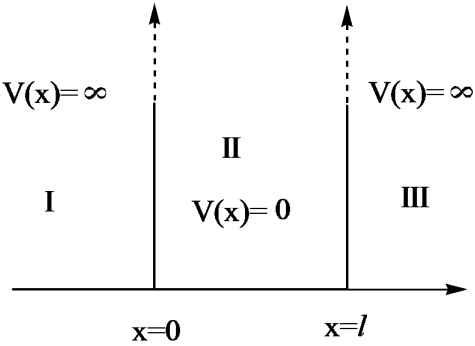
\includegraphics[scale=0.5]{fig/lzhx/微信图片_20211025092646.png}
\end{center}
我们给定一维势箱,粒子的势能$V(x)$为分段函数:
\[V(x)=\left \{
\begin{array}{rl}
+\infty & x<0\\
0 & 0 \leq x \leq l\\
+\infty & x>l
\end{array} \right .\]

由薛定谔方程,我们可以变形得到:
\[-\frac{\hbar^2}{2m}\nabla^2\varPsi+V\varPsi=E\varPsi\]
\[\varPsi=\frac{\hbar^2}{2m(V-E)}\nabla^2\varPsi\]

显然,我们能得到:
\[\lim_{V \rightarrow +\infty}\varPsi=0\]

因此,粒子波函数只可能出现在$x \in [0,l]$的范围内,
且为保证连续性,波函数还需满足满足下列边界条件,在这种意义下势箱波函数可以看成是一种驻波:
\[\varPsi(0)=0 \qquad \varPsi(l)=0\]

边界条件的引入也就是梦开始的地方,我们在自由粒子中看不到任何跟量子化有关系的地方,但是在接下来的内容以及后续的内容中我们会发现,
量子化的出现都不是来源于量子力学的基本方程也即薛定谔方程,而是来源于各种的边界条件:

利用边界条件$\varPsi(0)=0$:
\[\varPsi(0)=C_1sin \ 0+C_2cos \ 0=0 \Rightarrow C_2=0\]

再利用边界条件$\varPsi(l)=0$,我们得到一维势箱能量量子化:
\[\varPsi(l)=C_1sin(\frac{\sqrt{2mE}}{\hbar}l)=0 \Rightarrow E=\frac{n^2 \pi^2 \hbar^2}{2ml^2}=\frac{n^2 h^2}{8ml^2}\]

归一化:
\[\int_0^l\varPsi^*\varPsi=C_1^2\int_0^lsin^2\left (\frac{n \pi}{l}x \right )dx=\frac{C_1^2}{2}\int_0^l\left ( 1-cos\left (\frac{2n \pi}{l}x \right ) \right )dx=\frac{C_1^2l}{2}=1\]

故:
\[C_1=\sqrt{\frac{2}{l}}\]

最终我们得到归一化一维势箱波函数及能量表达式:
\[\varPsi_n=\sqrt{\frac{2}{l}}sin\left (\frac{n \pi}{l}x \right ) \qquad E_n=\frac{n^2 h^2}{8ml^2} \qquad (n=1,2,3 \cdots)\]

\begin{center}
    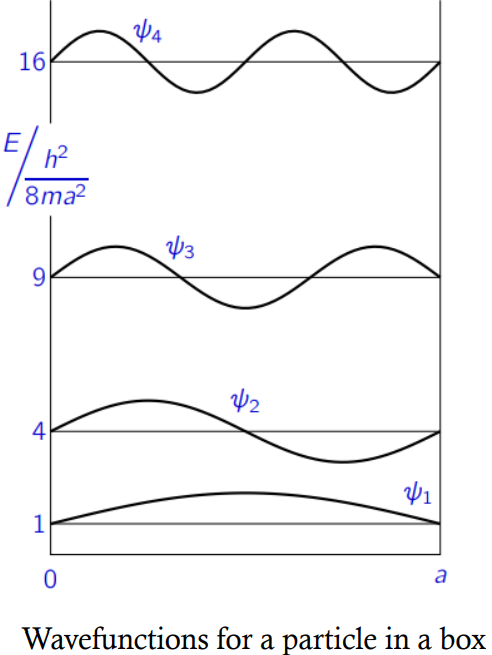
\includegraphics[scale=0.5]{fig/lzhx/微信图片_20211025150139.png}
\end{center}

\subsection{三维势箱Box[a,b,c]}
三维势箱在利用分离变量的方法可以看成三个一维势箱的乘积,这里我们简单介绍一下分离变量法在势箱中的应用,假设三维势箱三个坐标相互独立,则三维势箱波函数可以写成:
\[\varPsi(x,y,z):=X(x)Y(y)Z(z)\]
则,不考虑边界点,势箱波函数可以写成:
\[-\frac{\hbar^2}{2m}\nabla^2\varPsi=-\frac{\hbar^2}{2m}\left (YZ\frac{\partial^2X}{\partial x^2}+XZ\frac{\partial^2Y}{\partial y^2}+XY\frac{\partial^2Z}{\partial z^2} \right )=EXYZ\]

显然,除了平凡解$\psi=0$外,我们可以认为解出的波函数仅在有限个点上取值为零,不考虑这些奇异点,我们将方程两边同时除以$XYZ$:
\[-\frac{\hbar^2}{2m}\left (\frac{1}{X}\frac{\partial^2X}{\partial x^2}+\frac{1}{Y}\frac{\partial{d}^2Y}{\partial y^2}+\frac{1}{Z}\frac{\partial^2Z}{\partial z^2} \right )=E\]

同样的,我们定义:
\[E:=E_x+E_y+E_z\]

因此,我们可以将上述三维势箱薛定谔方程方程写成三个一维势箱薛定谔方程:
\[-\frac{\hbar^2}{2m}\frac{\mathrm{d}^2X}{\mathrm{d}x^2}=E_xX \qquad -\frac{\hbar^2}{2m}\frac{\mathrm{d}^2Y}{\mathrm{d}y^2}=E_yY \qquad -\frac{\hbar^2}{2m}\frac{\mathrm{d}^2Z}{\mathrm{d}z^2}=E_zZ\]

解得三个波函数及能量:
\[X=\sqrt{\frac{2}{a}}sin\left (\frac{n_x \pi}{l}x \right ) \qquad Y=\sqrt{\frac{2}{b}}sin\left (\frac{n_y \pi}{l}y \right ) \qquad Z=\sqrt{\frac{2}{c}}sin\left (\frac{n_z \pi}{l}z \right )\]
\[E_{x,n}=\frac{n_x^2 h^2}{8ma^2} \qquad E_{y,n}=\frac{n_y^2 h^2}{8mb^2} \qquad E_{z,n}=\frac{n_z^2 h^2}{8mc^2}\]
\[(n_x,n_y,n_z=1,2,3 \cdots)\]

合并波函数及能量:
\[\varPsi=\sqrt{\frac{8}{abc}}sin\left (\frac{n_x \pi}{l}x \right )sin\left (\frac{n_y \pi}{l}y \right )sin\left (\frac{n_z \pi}{l}z \right )\]
\[E_{x,n}=\frac{h^2}{8m} \left (\frac{n_x^2}{a^2}+\frac{n_y^2}{b^2}+\frac{n_z^2}{c^2} \right )\]
\[(n_x,n_y,n_z=1,2,3 \cdots)\]

\section{振动量子化——谐振子}
对势箱中的振动系统,我们可以把哈密顿量构造成:
\[\hat{H}=-\frac{\hbar^2}{2m_1}\nabla^2_1-\frac{\hbar^2}{2m_2}\nabla^2_2+V\]

对势能部分$V(r)$(内坐标表示),我们在平衡位置进行泰勒展开:
\[V(r)=V(r_e)+V^{'}(r)(r-r_e)+\frac{1}{2}V^{''}(r)(r-r_e)^2+\frac{1}{6}V^{'''}(r)(r-r_e)^3 \cdots=\sum_{i=0}^{+\infty}\frac{V^{(i)}(r_e)}{i!}(r-r_e)^i\]

对谐振子系统,其势能项可以为:
\[V(r)=V(r_e)+\frac{1}{2}V^{''}(r)(r-r_e)^2\]

因此,势箱中的谐振子薛定谔方程可以描述为:
\[\left (-\frac{\hbar^2}{2m_1}\nabla^2_1-\frac{\hbar^2}{2m_2}\nabla^2_2+V(r_e)+\frac{1}{2}V^{''}(r)(r-r_e)^2 \right )\varPsi=E\varPsi\]
考虑质心系
\[\left (-\frac{\hbar^2}{2\mu}\nabla^2+V(r_e)+\frac{1}{2}V^{''}(r)(r-r_e)^2 \right )\varPsi=E\varPsi\]

这里,我们不再求解该方程,有兴趣的可以自己上网查,这边直接给出解的形式:

则,解为:
\[\varPsi_n(x)=\left(\frac{\mu\omega}{\pi\hbar}\right)^{\frac{1}{4}}\frac{1}{\sqrt{2^nn!}}H_n(\sqrt{\frac{\mu\omega}{\hbar}}x)exp\left(-\frac{\mu\omega}{2\hbar}x^2\right) \qquad (n=1,2,3 \cdots)\]

能量为:
\[E_n=\left(n+\frac{1}{2}\right)h\nu=\left(n+\frac{1}{2}\right)\hbar\omega \qquad (n=1,2,3\cdots)\]

其中:
\[H_n(q)=(-1)^ne^{q^2}\frac{\mathrm{d}}{\mathrm{d}x}e^{-q^2} \qquad (n=1,2,3\cdots)\]
\[H_0(q)=1 \qquad H_1(q)=2q \qquad H_2(q)=4q^2-2\]
\[\omega=\sqrt{\frac{k}{\mu}}\]

当然,对一般的振动系统,谐振子近似经常是不够的,这时我们会引入非谐校正,比如,引入$Morse \ potential$:
\[V(r)=D_e\left[1-e^{-\beta(r-r_e)}\right]^2\]

同样对其进行展开得到:
\[V(r)=D_e\left[\beta^2(r-r_e)^2-\beta^3(r-r_e)^3+\cdots\right]\]

因此,对应于谐振子的力常数$k$有如下关系:
\[k=2\beta^2D_e\]

其能量可以用以下表达式给出:
\[E_\nu=\left(\nu+\frac{1}{2}\right)\hbar\omega-\left(\nu+\frac{1}{2}\right)^2\hbar\omega x_e \qquad x_e=\frac{\hbar\beta^2}{2\mu\omega}=\frac{\hbar\omega}{4D_e}\]

\begin{center}
    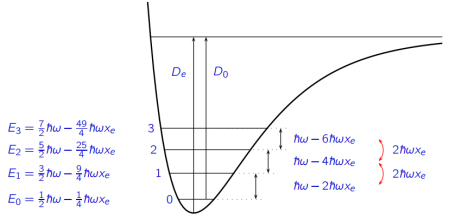
\includegraphics[scale=0.7]{fig/lzhx/微信图片_20211104112141.png}
\end{center}

\section{转动量子化——刚性转子}
由之前的讨论,我们知道,一个粒子的哈密顿量可以表示成:
\[\hat{H}=-\frac{\hbar^2}{2m}\nabla^2 + V=-\frac{\hbar^2}{2m}\left ( \frac{\partial^2}{\partial x^2}+\frac{\partial^2}{\partial y^2}+\frac{\partial^2}{\partial z^2}\right ) + V\]

因此,我们可以考虑两个粒子组成的刚性转子哈密顿量为:
\[\hat{H}=-\frac{\hbar^2}{2m}\left ( \frac{\partial^2}{\partial x_2^2}+\frac{\partial^2}{\partial y_2^2}+\frac{\partial^2}{\partial z_2^2}\right ) -\frac{\hbar^2}{2m}\left ( \frac{\partial^2}{\partial x_2^2}+\frac{\partial^2}{\partial y_2^2}+\frac{\partial^2}{\partial z_2^2}\right ) + V_{12}\]

考虑势箱中的刚性转子,$V_{12}=0$:
\[\hat{H}=-\frac{\hbar^2}{2m}\left ( \frac{\partial^2}{\partial x_1^2}+\frac{\partial^2}{\partial y_1^2}+\frac{\partial^2}{\partial z_1^2}\right ) -\frac{\hbar^2}{2m}\left ( \frac{\partial^2}{\partial x_2^2}+\frac{\partial^2}{\partial y_2^2}+\frac{\partial^2}{\partial z_2^2}\right )\]

定义内坐标:
\[ \left \{
    \begin{array}{ll}
        x=x_1-x_2  \\
        y=y_1-y_2  \\
        z=z_1-z_2
    \end{array}
    \right .
\]

则刚性转子的哈密顿量可以写成:
\[\hat{H}=-\frac{\hbar^2}{2}\left (\frac{1}{m_1}+\frac{1}{m_2}\right )\left ( \frac{\partial^2}{\partial x^2}+\frac{\partial^2}{\partial y^2}+\frac{\partial^2}{\partial z^2}\right )=-\frac{\hbar^2}{2\mu}\left ( \frac{\partial^2}{\partial x^2}+\frac{\partial^2}{\partial y^2}+\frac{\partial^2}{\partial z^2}\right ) \]

在球坐标下展开:
\[\hat{H}=-\frac{\hbar^2}{2\mu} \left (\frac{1}{r^2}\frac{\partial}{\partial{r}}(r^2\frac{\partial}{\partial{r}})+\frac{1}{r^2sin\theta}\frac{\partial}{\partial{\theta}}(sin\theta\frac{\partial}{\partial{\theta}})+\frac{1}{r^2sin^2 \theta }\frac{\partial^2}{\partial{\phi^2}} \right )\]

已知其中$r$为常数,则哈密顿量可以继续简化成:
\[\hat{H}=-\frac{\hbar^2}{2\mu} \left (\frac{1}{r^2sin\theta}\frac{\partial}{\partial{\theta}}(sin\theta\frac{\partial}{\partial{\theta}})+\frac{1}{r^2sin^2 \theta }\frac{\partial^2}{\partial{\phi^2}} \right )\]

将哈密顿量对波函数作用,我们稍作变形:
\[\hat{H}\varPsi=-\frac{\hbar^2}{2\mu} \left (\frac{1}{r^2sin\theta}\frac{\partial}{\partial{\theta}}(sin\theta\frac{\partial}{\partial{\theta}})+\frac{1}{r^2sin^2 \theta }\frac{\partial^2}{\partial{\phi^2}} \right )\varPsi=E\varPsi\]
\[-\hbar^2\left (\frac{1}{sin\theta}\frac{\partial}{\partial{\theta}}(sin\theta\frac{\partial}{\partial{\theta}})+\frac{1}{sin^2 \theta }\frac{\partial^2}{\partial{\phi^2}} \right )\varPsi=2\mu r^2 E\varPsi\]

稍微回顾一下经典力学,考虑两个质点$m_1$、$m_2$和轻轴组成的刚性旋转子,两质点间距为r,则此系统的质心系坐标、转动惯量和角动量及能量可以表示成:
\[r_1=\frac{m_2}{m_1+m_2}r \qquad r_2=\frac{m_1}{m_1+m_2}r\]
\[I=I_1+I_2=m_1r_1^2+m_2r_2^2=\frac{m_1m_2}{m_1+m_2}r^2\]
\[L=I\omega \qquad E=\frac{1}{2}I\omega^2=\frac{L^2}{2I}\]

则,我们可以将上述薛定谔方程改写成:
\[-\hbar^2\left (\frac{1}{sin\theta}\frac{\partial}{\partial{\theta}}(sin\theta\frac{\partial}{\partial{\theta}})+\frac{1}{sin^2 \theta }\frac{\partial^2}{\partial{\phi^2}} \right )\varPsi=L^2\varPsi\]

定义角动量平方算符,它反映的是波函数在空间中的角度部分延展程度:
\[\hat{J}^2=-\hbar^2\left (\frac{1}{sin\theta}\frac{\partial}{\partial{\theta}}(sin\theta\frac{\partial}{\partial{\theta}})+\frac{1}{sin^2 \theta }\frac{\partial^2}{\partial{\phi^2}} \right )\]

因此有:
\[\hat{J}^2\varPsi=L^2\varPsi\]

如果我们去解这个方程,我们会得到(我爬了,我实在不想再解一遍,想看的自己去附录求解氢原子薛定谔方程里找类似的部分,这里提供两个解的思路:一是级数法解微分方程,另外是利用升降算符):
\[\hat{J}^2\varPsi=l(l+1)\hbar^2\varPsi\]

其中$l$为角量子数。

当然,既然有了$\hat{J}^2$利用角动量模的平方表征波函数的角度部分,当然也会有利用角动量在某方向上的投影表征波函数的角度部分的算符,我们取投影方向为z:
\[\hat{J_z}\varPsi=l\hbar\varPsi\]

值得一提的是,量子力学中大部分算符是延用经典力学的算符,比如角动量算符可以通过$J=r \times p$得到。
 
\begin{center}
    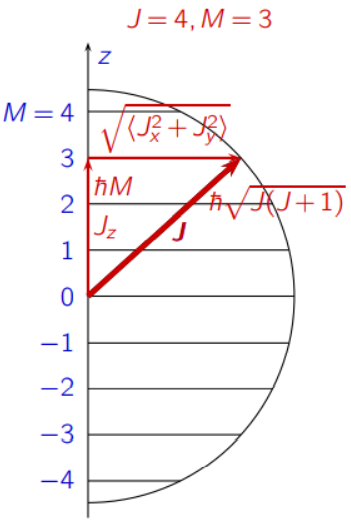
\includegraphics[scale=0.5]{fig/lzhx/微信图片_20211026130340.png}
\end{center}

\section{氢原子}
\subsection{氢原子薛定谔方程求解}
想看自己看附录I

\subsection{实、复轨道?}
举个例子,求解氢原子薛定谔方程我们能得到$n=2$,$l=1$,$m=-1,0,1$三个轨道波函数的表达式:
\[2p_0=N_{2p}ze^{-\frac{r}{2}} \qquad (m=0)\]
\[2p_1=-N_{2p}\frac{\sqrt{2}}{2}(x+iy)e^{-\frac{r}{2}} \qquad (m=1) \]
\[2p_{-1}=N_{2p}\frac{\sqrt{2}}{2}(x-iy)e^{-\frac{r}{2}} \qquad (m=-1) \]

这些轨道与我们所熟知的$2p_x,2p_y,2p_z$有如下关系:
\[2p_z=2p_0=N_{2p}ze^{-\frac{r}{2}} \quad 2p_x=\frac{\sqrt{2}}{2}(2p_{-1}-2p_1)=N_{2p}xe^{-\frac{r}{2}} \quad 2p_y=\frac{\sqrt{2}i}{2}(2p_{-1}+2p_1)=N_{2p}ye^{-\frac{r}{2}}\]

插句题外话,由于能量简并,这几个轨道的线性组合得到的任意波函数都是哈密顿量的本征函数,如果轨道能量不简并的话,轨道线性组合的结果将并不会是哈密顿量的本征函数(具体理由详见线性代数),其对算符作用后得到的也不是本征值而是平均值。

\section{单核多电子体系}
\subsection{波恩-奥本海默近似}
理论上对于一个微观体系,只要我们确定了粒子组成及其相互作用,我们就能写出该体系的哈密顿量,利用基本假设薛定谔方程去求解体系的波函数。
但是实际上你解个氢原子都解得要死要活的了,甚至氢分子你都不能精确解(这里指给出解析解,理论上来说只要你数值解的精度无穷大也可以认为是给出了精确解,但显然做不到),那么引入一些近似在不降低太多准确度的前提下大幅提高计算的速度就显得尤为重要。

这里我们介绍一个基本的也是最普遍的近似——波恩-奥本海默近似,至于为什么不是最基本的,等一下你就知道还有比他更底层的近似了。

哈密顿量可以写成动能部分和势能部分,那么我们还能继续拆下去吗,该怎么拆呢?一个自然而然的想法就是我们能不能把核的运动和电子的运动分离开呢?
于是我们就假设核跟电子的运动无关,进而可以将动能项拆成核动能部分和电子动能部分:
\[\hat{H}=\hat{T}+\hat{V} \qquad \hat{T}=\hat{T_n}+\hat{T_e}\]
于是在介绍波恩-奥本海默近似前我们其实用了一个更基本的近似。

结合上面的假设对一个分子体系,我们可以把哈密顿量写成:
\[\hat{H}=-\sum_i\frac{\hbar^2}{2m_{n,i}}\nabla^2_{n,i}-\sum_j\frac{\hbar^2}{2m_e}\nabla^2_{e,j}+\sum_{i,j}V_{i,j}\]

我们假设电子的波函数$\psi(Q,q)$和核的波函数$\varphi(Q)$可以分离,于是波函数可以写成如下形式,其中Q为核坐标,q为电子坐标:
\[\varPsi(Q,q)=\psi(Q,q)\varphi(Q)\]

正如波恩-奥本海默近似Born-Oppenheimer approximation的另一个名字定核近似,简单理解,电子相对于核运动太快,波恩-奥本海默近似就是认为核不动,当然这是不对的,波恩-奥本海默近似认为的是电子相较于原子核运动很快所以认为电子的总体分布在核外基本不变,所以有:
\[\nabla^2_n\psi(Q,q) \approx 0 \qquad \nabla_n\psi(Q,q) \approx 0\]

将哈密顿量作用在波函数上,先看动能部分:
\[\hat{T}\varPsi(Q,q)=-\sum_i\frac{\hbar^2}{2m_{n,i}}\nabla^2_{n,i}(\psi(Q,q)\varphi(Q))-\sum_j\frac{\hbar^2}{2m_e}\nabla^2_{e,j}(\psi(Q,q)\varphi(Q))\]

考虑核动能部分:
\[\hat{T_n}\varPsi(Q,q)=-\sum_i\frac{\hbar^2}{2m_{n,i}}\left (\nabla^2_{n,i}\psi(Q,q) \cdot \varphi(Q)+2\nabla_{n,i}\psi(Q,q) \cdot \nabla_{n,i}\varphi(Q)+ \psi(Q,q) \cdot \nabla^2_{n,i}\varphi(Q)  \right )\]
\[\hat{T_n}\varPsi(Q,q) \approx -\sum_i\frac{\hbar^2}{2m_{n,i}}\psi(Q,q) \cdot \nabla^2_{n,i}\varphi(Q)=-\psi(Q,q)\sum_i\frac{\hbar^2}{2m_{n,i}}\nabla^2_{n,i}\varphi(Q)\]

考虑电子动能部分:
\[\hat{T_e}\varPsi(Q,q)=-\varphi(Q)\sum_j\frac{\hbar^2}{2m_e}\nabla^2_{e,j}\psi(Q,q)\]

合并整个哈密顿量,可以将薛定谔方程改写成如下形式:
\[\hat{H}\varPsi=-\psi\sum_i\frac{\hbar^2}{2m_{n,i}}\nabla^2_{n,i}\varphi-\varphi\sum_j\frac{\hbar^2}{2m_e}\nabla^2_{e,j}\psi+\sum_{i,j}V_{i,j}\psi\varphi=E\psi\varphi\]

波恩-奥本海默近似其实也是一种分离变量,接下来的处理我们将不做多余的文字说明:
\[-\frac{1}{\varphi(Q)}\sum_i\frac{\hbar^2}{2m_{n,i}}\nabla^2_{n,i}\varphi(Q)-\frac{1}{\psi(Q,q)}\sum_j\frac{\hbar^2}{2m_e}\nabla^2_{e,j}\psi(Q,q)+\sum_{i,j}V_{i,j}=E\]
\[-\frac{1}{\varphi(Q)}\sum_i\frac{\hbar^2}{2m_{n,i}}\nabla^2_{n,i}\varphi(Q):=E-U(Q) \tag{a}\]
\[-\frac{1}{\psi(Q,q)}\sum_j\frac{\hbar^2}{2m_e}\nabla^2_{e,j}\psi(Q,q)+\sum_{i,j}V_{i,j}:=U(Q)\]
\[-\sum_j\frac{\hbar^2}{2m_e}\nabla^2_{e,j}\psi(Q,q)+\sum_{i,j}V_{i,j}\psi(Q,q)=U(Q)\psi(Q,q) \tag{b}\]

(a)式即为该分子体系的核薛定谔方程,(b)式即为该分子体系的电子薛定谔方程,也即我们遇见的最常见的薛定谔方程。顺便一提,重新定义的$U(Q)$即为Potential Energy Surface (PES),也即我们常说的势能面。
电子结构所关心的是(b)式,解出对应核构型下的电子分布,而动力学(化学反应)求解的是(a)式,认为给定核构型下的电子结构是已知的,某种意义上理论化学考虑化学反应是与电子无关的,这与某有机化学教授所说的"化学反应其实是电子的反应"相抵触(乐

一个有意思的事是,实际上我们求解氢原子的波函数时用的是只含电子项的薛定谔方程,但是我们依然说这个是精确解,这是为什么呢?
\textbf{因为波恩-奥本海默近似本质上是假定变量可分离,因此对实际上确实可分离的体系这就不是一种近似。}上述视角是从波函数出发,如果我们从哈密顿量开始看,波恩-奥本海默近实际上将核动能从电子哈密顿量中剔除,很容易被误认为是假设核不动。

\subsection{平均场近似}
至此,我们开始接触多电子体系,需要注意的是现在我们其实还是不能直接处理这样的多电子体系,主要的原因是电子-电子相互作用我们处理不了,所以我们需要考虑进一步近似把多电子体系近似成我们能处理的单电子体系。

考虑一个多电子原子,其电子哈密顿量可以表示成:
\[\hat{H}=-\sum_{i}\frac{\hbar^2}{2m_i}\nabla^2_i+\sum_{i,j}\frac{q_iq_j}{4 \pi \varepsilon_0 r_{ij}}-\sum_i\frac{q_iq_n}{4 \pi \varepsilon_0 r_{i}}\]

在平均场近似Central field approximation下,把其他电子对某电子的双体算符(势能)近似成其他电子对该电子产生的势场(单体算符),并且利用独立粒子近似Independent-particle approximation,把体系哈密顿量近似成单粒子哈密顿量的加和,其中$V_i$为其他粒子对第i个粒子产生的平均势场:
\[\hat{H}=\sum_{i}\hat{H}_{i} \qquad \text{where} \quad \hat{H}_i=-\frac{\hbar^2}{2m_i}+V_i\]

同理,电子波函数也近似成各个单电子波函数的乘积:
\[\varPsi=\prod_i\varPsi_i\]

利用分离变量法,我们将原体系总波函数写成单体波函数:
\[\hat{H}_i\varPsi_i=\left ( -\frac{\hbar^2}{2m_i}+V_i \right ) \varPsi_i=\varepsilon_i\varPsi_i\]

平均场近似下,我们一般配合自洽场方法Self-Consistent Field (SCF)进行求解,自洽场方法的基本思路是利用一套初始的猜测轨道计算势场$V_i$,然后将$V_i$代入方程重新计算轨道,然后不断迭代最终得到稳定解:

我们从电子1(只是我们人为的编号,不代表粒子是可区分的)开始:

某电子的电荷密度可以用下式描述:
\[\rho_i=-e|\varPsi_i|^2 \qquad (i=1,2,3 \cdots n)\]

其对电子1产生的势场为:
\[V_{1i}=\frac{-e}{4 \pi \varepsilon_0}\int_{\mathbb{R}^3}\frac{\rho_i}{r_{1i}}d\tau_i=\frac{e^2}{4 \pi \varepsilon_0}\int_{\mathbb{R}^3}\frac{|\varPsi_i|^2}{r_{1i}}d\tau_i \qquad (i=2,3,4 \cdots n)\]

故电子1受到的势场$V_1$为:
\[V_i=\sum_{i=2}^nV_{1i}-\frac{Ze^2}{4 \pi \varepsilon_0r_1}=\sum_{i=2}^n\frac{e^2}{4 \pi \varepsilon_0}\int_{\mathbb{R}^3}\frac{|\varPsi_i|^2}{r_{1i}}d\tau_i-\frac{Ze^2}{4 \pi \varepsilon_0r_1}\]

故,粒子1的单电子薛定谔方程可以构建成:
\[\left ( -\frac{\hbar^2}{2m_1}+V_1 \right ) \varPsi_1=\varepsilon_1\varPsi_1\]

求解该方程我们可以得到更新的轨道$\varPsi_1$,利用其我们可以进入粒子2的运算,如此往复一直迭代至收敛至稳定解。

\subsection{粒子全同性与泡利不相容原理}
全同性应该是微观粒子与宏观物体最不同的地方之一。

简单来说,对两个宏观物体A、B,除了速度、位置外,我们还有大小、颜色之类的特征作为区分物体A、B,这也即表面在经典物理框架下,并没有全同性这一说法。但对于微观粒子A、B,我们似乎只有速度和位置这类无法区分粒子的可观测量。

除了质量,电荷这种不能区分粒子的性质外,我们只知道微观粒子的自旋状态以及其所在的能级或者说单粒子空间轨道(如果我们认为多粒子波函数可以被单粒子波函数展开的话),可以合并两者成单粒子的自旋轨道,他同样也不能区分粒子。这就意味着你只能把一堆不可区分的粒子放在不同的状态上,\textbf{对同一类粒子(质量,电荷,总自旋角动量$S^2$)而言,你只能区分态而不能区分粒子本身}。你舌头上的电子跟野兽先辈林檎上的电子就是全同的。

相关的拓展内容可以请大家阅读一些关于“吉布斯佯谬”的相关论述,理解一些传统统计力学与量子统计力学的一些差异。

接下来,我们的表述将在全同性这一基本假设下展开。

首先定义对换算符$\hat{P}_{ij}$:
\[\hat{P}_{ij}\varPsi(\cdots,i,\cdots,j,\cdots)=\varPsi(\cdots,j,\cdots,i,\cdots)\]

基于全同性,就一个多粒子体系而言,我们调换一对同类型的粒子,显然其分布概率并不会被改变(有经典对应的物理量在埃伦费斯特定理(Ehrenfest's theorem)的保证下符合经典物理的行为,故在选取被观测量的时候我们会尽量选择有经典对应的物理量):
\[|\varPsi(\cdots,i,\cdots,j,\cdots)|^2=|\varPsi(\cdots,j,\cdots,i,\cdots)|^2\]
\[\varPsi(\cdots,i,\cdots,j,\cdots)=\pm\varPsi(\cdots,j,\cdots,i,\cdots)\]

依据上述描述,对换算符和哈密顿算符必然是对易的:
\[\qty[\hat{P}_{ij},\hat{H}]=0\]

对应,上述两种波函数行为,我们定义两类粒子——玻色子和费米子,玻色子函数对对换对称,费米子对对换反对称:
\[
    \begin{array}{lll}
        \text{Boson} & \varPsi(\cdots,i,\cdots,j,\cdots)=\varPsi(\cdots,j,\cdots,i,\cdots) & \text{symmetric} \\
        \text{Fermion} & \varPsi(\cdots,i,\cdots,j,\cdots)=-\varPsi(\cdots,j,\cdots,i,\cdots) & \text{antisymmetric}
    \end{array}
\]

玻色子自旋为整数,费米子自旋为半整数。

考虑电子,电子是费米子,所以电子的波函数应该是反对称的。

当然除了一次换电子,我们也可以考虑一次对换多个电子,我们将其记为$\hat{P}_k$,称为置换算符,在行列式的定义中其实已经用到过该算符。利用置换算符我们还可以构造对称算符$\hat{S}$以及反对称算符$\hat{A}$,其中$\tau$为任意n元排列$k$的逆序数,$k$的个数为$n!$:
\[\hat{S}=\frac{1}{\sqrt{n!}}\sum_{k}\hat{P}_{k} \qquad \hat{A}=\frac{1}{\sqrt{n!}}\sum_{k}(-1)^{\tau}\hat{P}_{k}\]

用这两个算符,我们可以构造出多满足泡利不相容原理的玻色子或费米子体系的波函数,以双粒子双能级体系为例,粒子用$1,2$区分,能级用$a,b$区分:
\[
    \begin{array}{ll}
        \text{Boson} & \hat{S}\varPsi_{ab}(1,2)=\frac{1}{\sqrt{2!}}[\varphi_a(1)\varphi_b(2)+\varphi_a(2)\varphi_b(1)]\\
        \text{Fermion} & \hat{A}\varPsi_{ab}(1,2)=\frac{1}{\sqrt{2!}}[\varphi_a(1)\varphi_b(2)-\varphi_a(2)\varphi_b(1)] 
    \end{array}
\]

考虑一件有意思的事情,如果所有粒子处于同一个量子态,玻色子和费米子会有什么样的行为?

我们这里继续使用上述的两个算符构造:
\[\hat{S}\varPsi_{1}(1,2,3 \cdots)=\frac{1}{\sqrt{n!}}\sum_{k}\hat{P}_{k}\varPsi_{1}(1,2,3 \cdots)=\frac{1}{\sqrt{n!}}\cdot n!\prod_{i=1}^n\varphi_1(i)=\sqrt{n!}\prod_{i=1}^n\varphi_1(i)\]
\[\hat{A}\varPsi_{1}(1,2,3 \cdots)=\frac{1}{\sqrt{n!}}\sum_{k}(-1)^{\tau}\hat{P}_{k}\varPsi_{1}(1,2,3 \cdots)=\frac{1}{\sqrt{n!}}\left (\frac{n!}{2}\prod_{i=1}^n\varphi_1(i)-\frac{n!}{2}\prod_{i=1}^n\varphi_1(i) \right )=0\]

这就是常听说的同态玻色子倾向于聚集而同态费米子倾向于远离的数学表述。

\subsection{电子自旋}
非相对论量子力学体系下,电子自旋被认为是电子的内禀性质,强行跟轨道角动量类比得到:

\[
    \begin{array}{ll}
        \hat{J}(\hat{J_x},\hat{J_y},\hat{J_z}) & \hat{S}(\hat{S_x},\hat{S_y},\hat{S_z}) \\
        L=\sqrt{l(l+1)}\hbar & S=\sqrt{s(s+1)}\\
        i=0,1,2 \cdots & s=\frac{1}{2}\\
        J_z=m_l\hbar & S_z=m_s\hbar\\
        m_l - \text{magnetic number}, & m_s - \text{magnetic spin number},\\
        \hat{J}^2=\hat{J_x}^2+\hat{J_y}^2+\hat{J_z}^2 & \hat{S}^2=\hat{S_x}^2+\hat{S_y}^2+\hat{S_z}^2 \\
        \qty[\hat{J}^2,\hat{J_n}]=0 \ (n=x,y,z) & \qty[\hat{S}^2,\hat{S_n}]=0 \ (n=x,y,z)\\
        \qty[\hat{J_x},\hat{J_y}]=i\hbar\hat{J_z} & \qty[\hat{S_x},\hat{S_y}]=i\hbar\hat{S_z}\\
        \qty[\hat{J_z},\hat{J_x}]=i\hbar\hat{J_y} & \qty[\hat{S_z},\hat{S_x}]=i\hbar\hat{S_y}\\
        \qty[\hat{J_y},\hat{J_z}]=i\hbar\hat{J_x} & \qty[\hat{S_y},\hat{S_z}]=i\hbar\hat{S_x}
    \end{array}
\]

虽然电子的自旋被认为是电子场的自然结论,但我们不打算在这里介绍相对论量子力学(我暂时也不会)。
本小节我们只介绍电子自旋的一些物理性质并讨论其部分算符以及可观测量,在下一章节我们会介绍电子自旋对原子的物理性质如光谱的影响。

\begin{center}
    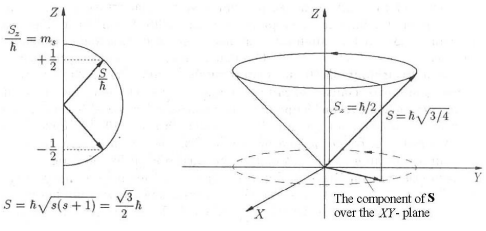
\includegraphics[scale=0.7]{fig/lzhx/微信图片_20211028113518}
\end{center}

总结一下我们至今碰到的算符,这里我们采用量子数形式的狄拉克表示符号代替波函数:
\[
    \begin{array}{ll}
        \ket{nlm_lm_s}=R_{nl}(r)Y_{l,m_l}(\theta,\varphi)\sigma_{m_s} \\
        \hat{H}\ket{nlm_lm_s}=E_{nl}\ket{nlm_lm_s} \\
        \hat{J}^2\ket{nlm_lm_s}=l(l+1)\hbar^2\ket{nlm_lm_s} \\
        \hat{J_z}\ket{nlm_lm_s}=m_l\hbar\ket{nlm_lm_s} \\
        \hat{S}^2\ket{nlm_lm_s}=s(s+1)\hbar^2\ket{nlm_lm_s} \\
        \hat{S_z}\ket{nlm_lm_s}=m_s\hbar\ket{nlm_lm_s}
    \end{array}
\]

如果我们对一个双电子体系进行考察,其自旋可以采用如下四种状态:
\[\sigma_{12}=\sigma_{1}\sigma_{2}=\alpha_1\alpha_2, \ \alpha_1\beta_2, \ \beta_1\alpha_2, \ \beta_1\beta_2\]

我们定义该体系的总自旋角动量z投影算符为:
\[\hat{S}_z=\hat{S}_{1z}+\hat{S}_{2z}\]

将其作用在该体系上:
\[\hat{S_z}\sigma_{12}=\hat{S_{1z}}\sigma_{1}\sigma_{2}+\hat{S_{2z}}\sigma_{1}\sigma_{2}=(m_{s1}+m_{s2})\sigma_{12}:=M_s\sigma_{12}\]

显然$M_s$可以取值$-1,0,1$,分别对应正交归一化波函数:
\[
    \left \{
    \begin{array}{ll}
        M_s=1  & \sigma_{12}=\alpha_1\alpha_2\\
        M_s=0  & \sigma_{12}=\alpha_1\beta_2,\beta_1\alpha_2\\
        M_s=-1 & \sigma_{12}=\beta_1\beta_2
    \end{array}
    \right .
\]

但总感觉上式有什么不对的地方。我们会发现当$M_s=0$时出现的自旋波函数对称性不满足我们在全同性中给出的要求(不对称的乘上什么都是不对称的),为此,我们需要讲这两个波函数进行线性组合使之满足对称性及归一化的要求,组合的合理性详见线性代数关于简并特征值的描述。

关于归一化,我们在这里补充一点说明,由于电子自旋假设,电子波函数可以写成,其中$\varphi$为轨道波函数,$\sigma$为自旋波函数,在之前的章节中,我们已经介绍了轨道波函数是归一的:
\[\varPsi=\varphi\sigma\]

介绍一种简单的表示方法——狄拉克表示:
\[
    \left \{
    \begin{array}{l}
        \bra{\varPsi}:=\varPsi^{*} \\
        \ket{\varPsi}:=\varPsi \\
        \bra{\varPsi}\hat{H}\ket{\varPsi}:=\int_E \varPsi^{*}\hat{H}\varPsi d\tau \\
        \bra{\varPsi}\ket{\varPsi}:=\int_E \varPsi^{*}\varPsi d\tau 
    \end{array} 
    \right .
\]
\[\bra{\varPsi}\ket{\varPsi}=\bra{\varphi\sigma}\ket{\varphi\sigma}=\bra{\varphi}\ket{\varphi}\bra{\sigma}\ket{\sigma}=1 \cdot 1=1\]

回到上述问题,我们假设:
\[\sigma_{0,1}=C_1\alpha_1\beta_2+C_2\beta_1\alpha_2 \qquad (C_1,C_2 \in \mathbb{R})\]

并构造$\sigma_{0,1}$的正交向量$\sigma_{0,2}$,在$\alpha_1\beta_2,\beta_1\alpha_2$张成的二维空间中,与$\sigma_{0,1}$正交的向量有且只有:
\[\sigma_{0,2}= \pm (C_1\alpha_1\beta_2-C_2\beta_1\alpha_2)\]

考虑常数的任意性,不妨取:
\[\sigma_{0,2}= C_1\alpha_1\beta_2-C_2\beta_1\alpha_2\]

$\sigma_{0,1}$、$\sigma_{0,2}$满足条件:
\[\bra{\sigma_{0,i}}\ket{\sigma_{0,i}}=C_1^2\bra{\alpha_1\beta_2}\ket{\alpha_1\beta_2}+C_2^2\bra{\beta_1\alpha_2}\ket{\beta_1\alpha_2}+2C_1C_2\bra{\alpha_1\beta_2}\ket{\beta_1\alpha_2}=C_1^2+C_2^2=1 \qquad (i=1,2)\]
\[\bra{\sigma_{0,1}}\ket{\sigma_{0,2}}=C_1^2\bra{\alpha_1\beta_2}\ket{\alpha_1\beta_2}-C_2^2\bra{\beta_1\alpha_2}\ket{\beta_1\alpha_2}=C_1^2-C_2^2=0\]

取系数$C_1$、$C_2$为正,得到:
\[\sigma_{0,1}=\frac{1}{\sqrt{2}}(\alpha_1\beta_2+\beta_1\alpha_2) \qquad \sigma_{0,2}= \frac{1}{\sqrt{2}}(\alpha_1\beta_2-\beta_1\alpha_2)\]

故$M_s$取值$-1,0,1$分别对应正交归一化波函数为:
\[ 
    \left \{
    \begin{array}{ll}
        M_s=1  & \sigma_{12}=\alpha_1\alpha_2\\
        M_s=0  & \sigma_{12}=\frac{1}{\sqrt{2}}(\alpha_1\beta_2+\beta_1\alpha_2),\frac{1}{\sqrt{2}}(\alpha_1\beta_2-\beta_1\alpha_2)\\
        M_s=-1 & \sigma_{12}=\beta_1\beta_2
    \end{array}
    \right .
\]
考虑对称性,我们可以讲上述四个轨道分为两类:
\[ 
    \begin{array}{ll}
        \text{symmetric}: & \text{antisymmetric}: \\
         \alpha_1\alpha_2\\
         \frac{1}{\sqrt{2}}(\alpha_1\beta_2+\beta_1\alpha_2) & \frac{1}{\sqrt{2}}(\alpha_1\beta_2-\beta_1\alpha_2)\\
         \beta_1\beta_2
    \end{array}
\]

类似于上述的讨论,关于双粒子的轨道波函数,我们也能构造出对称于反对称的正交归一波函数:
\[
    \begin{array}{ll}
        \text{symmetric}: & \text{antisymmetric}: \\
        \frac{1}{\sqrt{2!}}[\varphi_a(1)\varphi_b(2)+\varphi_a(2)\varphi_b(1)] & \frac{1}{\sqrt{2!}}[\varphi_a(1)\varphi_b(2)-\varphi_a(2)\varphi_b(1)] 
    \end{array}
\]

将两者组合,为满足电子波函数反对称化的要求,我们只能这么组合:
\[
    \begin{array}{l}
        \varPsi_{singlet}=\frac{1}{\sqrt{2!}}[\varphi_a(1)\varphi_b(2)+\varphi_a(2)\varphi_b(1)]\times\frac{1}{\sqrt{2}}(\alpha_1\beta_2-\beta_1\alpha_2)\\
        \varPsi_{triplet}=\frac{1}{\sqrt{2!}}[\varphi_a(1)\varphi_b(2)-\varphi_a(2)\varphi_b(1)]\times \left \{
            \begin{array}{l}
                \alpha_1\alpha_2\\
                \frac{1}{\sqrt{2}}(\alpha_1\beta_2+\beta_1\alpha_2)\\
                \beta_1\beta_2
            \end{array}
        \right .
    \end{array}
\]

至此,我们也顺便组合出了单重态和三重态的电子波函数。

\subsection{slater行列式}
slater行列式是一种构造反对称波函数的表示方式,这里以锂原子为例,数字为电子编号,其slater行列式为:
\[\varPhi=\frac{1}{\sqrt{n!}}
\left |
\begin{array}{lll}
1s(1)\alpha(1) & 1s(1)\beta(1) & 2s(1)\alpha(1) \\
1s(2)\alpha(2) & 1s(2)\beta(2) & 2s(1)\alpha(2) \\
1s(1)\alpha(3) & 1s(1)\beta(3) & 2s(1)\alpha(3)
\end{array}
\right |
=\frac{1}{\sqrt{n!}}
\left |
\begin{array}{lll}
1s(1) & \overline{1s(1)} & 2s(1) \\
1s(2) & \overline{1s(2)} & 2s(2) \\
1s(3) & \overline{1s(3)} & 2s(3)
\end{array}
\right |
\]

或者,我们可以换一种更简洁的表示方式:
\[\varPhi=\hat{A}\varPsi_{a_1,a_2,a_3 \cdots}(1,2,3\cdots)=\frac{1}{\sqrt{n!}}\sum_k(-1)^{\tau}\varPsi_{a_k}(k)\]

\subsection{氦原子}
根据上面的讨论,我们可以得到氦原子的$1s2s$激发单重态轨道波函数:
\[\varPsi_{+}=\frac{1}{\sqrt{2!}}[\varphi_a(1)\varphi_b(2)+\varphi_a(2)\varphi_b(1)]\]

久违地考虑一下能量,写出氦原子的电子哈密顿算符:
\[\hat{H}=-\sum_{i=1}^2\frac{\hbar^2}{2m_e}\nabla^2_i-\sum_{i=1}^2\frac{e^2}{2 \pi \varepsilon_0 r_{i}}+\frac{e^2}{4 \pi \varepsilon_0 r_{12}}\]

定义,球形势场下的单电子体系哈密顿算符为$\hat{h}$与能量$\varepsilon$,由之前的讨论我们知道该体系是可以精确求解的(下面的运算均在原子单位下表示,简洁):
\[E=\bra{\varPsi_{+}}\hat{H}\ket{\varPsi_{+}}=\bra{\varPsi_{+}}\hat{h}_1\ket{\varPsi_{+}}+\bra{\varPsi_{+}}\hat{h}_2\ket{\varPsi_{+}}+\bra{\varPsi_{+}}\frac{1}{r_{12}}\ket{\varPsi_{+}}=2\varepsilon_{1}+\bra{\varPsi_{+}}\frac{1}{r_{12}}\ket{\varPsi_{+}}\]

可以发现,阻止我们精确求解多电子体系的主要障碍来源于电子——电子相互作用项:
\[\bra{\varPsi_{+}}\frac{1}{r_{12}}\ket{\varPsi_{+}}\]

更准确的说是轨道——轨道相互作用,因为电子自旋部分与积分坐标无关且正交归一:
\[\bra{\varPsi_{+}}\frac{1}{r_{12}}\ket{\varPsi_{+}}=\bra{\varphi_{+}\sigma_{singlet}}\frac{1}{r_{12}}\ket{\varphi_{+}\sigma_{singlet}}=\bra{\varphi_{+}}\frac{1}{r_{12}}\ket{\varphi_{+}}\bra{\sigma_{singlet}}\ket{\sigma_{singlet}}=\bra{\varphi_{+}}\frac{1}{r_{12}}\ket{\varphi_{+}}\]

具体来看它:
\[\bra{\varphi_{+}}\frac{1}{r_{12}}\ket{\varphi_{+}}=\frac{1}{2}\int_{\mathbb{R}^{3 \times 2}}[\varphi_a(1)\varphi_b(2)+\varphi_a(2)\varphi_b(1)]^{*}\frac{1}{r_{12}}[\varphi_a(1)\varphi_b(2)+\varphi_a(2)\varphi_b(1)]d\tau_1d\tau_2\]
\[\bra{\varphi_{+}}\frac{1}{r_{12}}\ket{\varphi_{+}}=\int_{\mathbb{R}^{3 \times 2}} \left ( [\varphi_a(1)\varphi_b(2)]^{*}\frac{1}{r_{12}}[\varphi_a(1)\varphi_b(2)]+[\varphi_a(1)\varphi_b(2)]^{*}\frac{1}{r_{12}}[\varphi_a(2)\varphi_b(1)] \right )d\tau_1d\tau_2\]

定义库伦积分$J$和交换积分$K$,显然这两个积分都是正的:
\[J:=\int_{\mathbb{R}^{3 \times 2}}[\varphi_a(1)\varphi_b(2)]^{*}\frac{1}{r_{12}}[\varphi_a(1)\varphi_b(2)]d\tau_1d\tau_2\]
\[K:=\int_{\mathbb{R}^{3 \times 2}}[\varphi_a(1)\varphi_b(2)]^{*}\frac{1}{r_{12}}[\varphi_a(2)\varphi_b(1)]d\tau_1d\tau_2\]

可以看出,库伦积分与经典物理中的定义相符,而交换积分更像是经典物理中“凭空冒出来”的。

最后,我们得到:
\[\bra{\varPsi_{+}}\frac{1}{r_{12}}\ket{\varPsi_{+}}=J+K\]

对三重态:
\[\varPsi_{-}=\frac{1}{\sqrt{2!}}[\varphi_a(1)\varphi_b(2)-\varphi_a(2)\varphi_b(1)]\]

同理有:
\[\bra{\varPsi_{-}}\frac{1}{r_{12}}\ket{\varPsi_{-}}=J-K\]

可见同电子排布下,三重态能量一般是要比单重态低,验证洪特规则。

观察三重态和单重态波函数分布概率对$r_{12}$变化的行为:
\begin{center}
    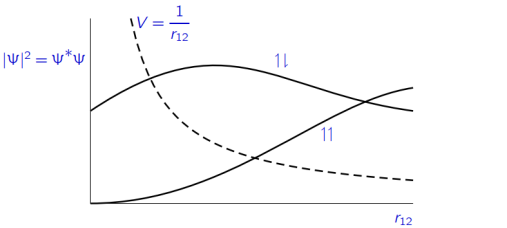
\includegraphics[scale=0.8]{fig/lzhx/微信图片_20211030111438.png}
\end{center}

在7.3中我们已经介绍了当$r_{12}=0$时的情况,三重态电子在$r_{12}=0$时分布概率为0,且从图像上来看,自旋平行的电子在空间上倾向于相互远离。而单重态电子在$r_{12}=0$时仍有分布,最大分布概率对应的$r_{12}$存在,也即我们一般认识的轨道半径。三重态在$r_{12}=0$的情况被称作Fermi hole。

\section{原子光谱}
对于原子的实际哈密顿量$\hat{H}$,我们可以把它拆成以下三个部分:平均场近似下的$\hat{H}_0$,平均场近似带来的与实际哈密顿量的势能误差项$\hat{H}^{'}$,以及填入电子后电子自旋与轨道自旋耦合带来的哈密顿量$\hat{H}_{SO}$。
\[\hat{H_0}=-\frac{\hbar^2}{2m_e}\sum_i\nabla^2_i+\sum_iV_i\]
\[\hat{H}^{'}=\sum_{i,j}\frac{1}{r_{ij}}-\sum_iV_i\]
\[\hat{H}_{SO}=\sum_{i}\xi(r_i)\hat{L}_i \cdot \hat{S}_i\]

旋轨耦合来源于哪里?其源头来自于量子纠缠,在原子分子尺度下,组成其的微粒——原子核/电子的德布罗意波强烈耦合,波函数无法独立区分,体系的物理量不能通过每个粒子的物理量进行加和得到。
\[\Psi(x_1,x_2) \neq \psi(x_1)\psi(x_2) \qquad \hat{A}\Psi(x_1,x_2) \neq (\hat{A}_1+\hat{A}_2)\psi(x_1)\psi(x_2)=(a_1+a_2)\psi(x_1)\psi(x_2)\]

表示方法(光谱项,光谱支项):
\[^{2S+1}L \qquad ^{2S+1}L_J\]

其中:
\[S=\sum_i\overrightarrow{m_s}(i)\]
\[L=\sum_i\overrightarrow{m_l}(i)\]
\[\overrightarrow{J}=\overrightarrow{S}+\overrightarrow{L} \qquad J=L+S,L+S-1,\cdots |L-S|\]

光谱支项多重度:
\[(2S+1)(2L+1)\]

每个光谱支项的简并度:
\[m_j:=2J+1\]

\subsection{Hund规则}
1、同电子组态,S越大越稳定;

2、S相同,L越大越稳定;

3、L、S相同,若电子数小于半满,J越小越稳定;若电子数大于半满,J越大越稳定。

\section{多核粒子体系——线性变分法}
对一些复杂的多核粒子体系,我们没有办法通过精确求解薛定谔方程得到其能量与波函数,但是我们可以通过利用现有的精确求解波函数猜测其实际波函数的办法来近似实际体系。
一般而言自然体系都会倾向于使得某态的能量尽可能低,所以我们可以利用猜测轨道得到的能量来衡量近似的质量。
当然该不等式可能需要要求猜测波函数是正交归一的。
\[\expval{\tilde{E}}=\frac{\bra{\varPhi}\hat{H}\ket{\varPhi}}{\bra{\varPhi}\ket{\varPhi}} \geqslant E_0\]

这里介绍一下基于原子轨道线性组合(LCAO)得到的猜测分子波函数LCAO-MO进行变分的过程,选用线性组合主要也是因为运算简单。

利用态叠加原理,现定义猜测波函数$\varPhi$,下表达式中,$c_i$为系数,$f_i$为已知波函数,波函数组张成的空间称为变分空间:
\[\varPhi=\sum_ic_if_i\]

代入我们的判据:
\[\expval{\tilde{E}}=\frac{\sum_{i,j}c_ic_j\bra{f_i}\hat{H}\ket{f_j}}{\sum_{i,j}c_ic_j\bra{f_i}\ket{f_j}}\]

这里再定义几个符号:
\[H_{ij}:=\bra{f_i}\hat{H}\ket{f_j} \qquad S_{ij}:=\bra{f_i}\ket{f_j} \qquad \sum:=\sum_{i,j}\]

则:
\[\expval{\tilde{E}}=\frac{\sum c_ic_jH_{ij}}{\sum c_ic_jS_{ij}}\]

为了找到再已有函数下使得$\expval{\tilde{E}}$最小的系数组$c_i$,我们需要$\expval{\tilde{E}}$对系数组$c_i$的偏导值等于0,二阶偏导矩阵正定。

为方便处理,我们做以下变形:
\[\expval{\tilde{E}}\sum c_ic_jS_{ij}=\sum c_ic_jH_{ij}\]

对$c_i$求偏导:
\[\frac{\partial \expval{\tilde{E}}}{\partial c_i}\sum c_ic_jS_{ij}+2\expval{\tilde{E}}\sum_j c_jS_{ij}=2\sum_j c_jH_{ij}\]
\[\frac{\partial \expval{\tilde{E}}}{\partial c_i}=\frac{2}{\sum c_ic_jS_{ij}}\left(\sum_j c_jH_{ij}-\expval{\tilde{E}}\sum_j c_jS_{ij}\right)=\frac{2}{\sum c_ic_jS_{ij}}\left(\sum_j \left (H_{ij}-\expval{\tilde{E}}S_{ij}\right )c_j\right)\]
\[\frac{\partial \expval{\tilde{E}}}{\partial c_i}=0 \Leftrightarrow \sum_j \left (H_{ij}-\expval{\tilde{E}}S_{ij}\right )c_j=0 \qquad (i=1,2,3 \cdots)\]

合并上式:
\[
\begin{pmatrix}
H_{11}-\expval{\tilde{E}}S_{11} & H_{12}-\expval{\tilde{E}}S_{12} & \ldots & H_{1n}-\expval{\tilde{E}}S_{1n}\\
H_{21}-\expval{\tilde{E}}S_{21} & H_{22}-\expval{\tilde{E}}S_{22} & \ldots & H_{2n}-\expval{\tilde{E}}S_{2n}\\
\vdots & \vdots & \ddots & \vdots\\
H_{n1}-\expval{\tilde{E}}S_{n1} & H_{n2}-\expval{\tilde{E}}S_{n2} & \ldots & H_{nn}-\expval{\tilde{E}}S_{nn}\\
\end{pmatrix}
\begin{pmatrix}
c_1\\
c_2\\
\vdots\\
c_n\\
\end{pmatrix}
=0
\]

要使得上述齐次方程有解,需要其系数矩阵行列式为0:
\[
    \begin{vmatrix}
        H_{11}-\expval{\tilde{E}}S_{11} & H_{12}-\expval{\tilde{E}}S_{12} & \ldots & H_{1n}-\expval{\tilde{E}}S_{1n}\\
        H_{21}-\expval{\tilde{E}}S_{21} & H_{22}-\expval{\tilde{E}}S_{22} & \ldots & H_{2n}-\expval{\tilde{E}}S_{2n}\\
        \vdots & \vdots & \ddots & \vdots\\
        H_{n1}-\expval{\tilde{E}}S_{n1} & H_{n2}-\expval{\tilde{E}}S_{n2} & \ldots & H_{nn}-\expval{\tilde{E}}S_{nn}\\
    \end{vmatrix}
    =0
\]

求解上述行列式我们能得到能量的估计最小值$\expval{\tilde{E}}$。

下面举个例子,如果我们考虑两个波函数张成的变分空间的线性变分:
\[\varPhi=\sum_{i=1}^2c_if_i\]
\[\expval{\tilde{E}}=\frac{\sum c_ic_jH_{ij}}{\sum c_ic_jS_{ij}}\]
\[\expval{\tilde{E}}\sum_{i=1}^2 c_ic_jS_{ij}=\sum_{i=1}^2 c_ic_jH_{ij}\]

对$c_i$求偏导:
\[\frac{\partial \expval{\tilde{E}}}{\partial c_i}\sum c_ic_jS_{ij}+2\expval{\tilde{E}}\sum_{i=1}^2 c_jS_{ij}=2\sum_{i=1}^2 c_jH_{ij}\]
\[\frac{\partial \expval{\tilde{E}}}{\partial c_i}=\frac{2}{\sum c_ic_jS_{ij}}\left(\sum_{i=1}^2 c_jH_{ij}-\expval{\tilde{E}}\sum_{i=1}^2 c_jS_{ij}\right)=\frac{2}{\sum c_ic_jS_{ij}}\left(\sum_j \left (H_{ij}-\expval{\tilde{E}}S_{ij}\right )c_j\right)\]
\[\frac{\partial \expval{\tilde{E}}}{\partial c_i}=0 \Leftrightarrow \sum_{i=1}^2 \left (H_{ij}-\expval{\tilde{E}}S_{ij}\right )c_j=0 \qquad (i=1,2)\]
\[
\begin{pmatrix}
H_{11}-\expval{\tilde{E}}S_{11} & H_{12}-\expval{\tilde{E}}S_{12} \\
H_{21}-\expval{\tilde{E}}S_{21} & H_{22}-\expval{\tilde{E}}S_{22} \\
\end{pmatrix}
\begin{pmatrix}
c_1\\
c_2
\end{pmatrix}
=0
\]
\[
    \begin{vmatrix}
        H_{11}-\expval{\tilde{E}}S_{11} & H_{12}-\expval{\tilde{E}}S_{12} \\
        H_{21}-\expval{\tilde{E}}S_{21} & H_{22}-\expval{\tilde{E}}S_{22} \\
    \end{vmatrix}
    =0
\]

对同核双原子分子,重新定义几个符号:
\[\alpha:=H_{11}=H_{22} \qquad \beta:=H_{12}=H_{21} \qquad S:=S_{12}=S_{21} \qquad S_{11}=S_{22}=1\]
\[
    \begin{vmatrix}
        \alpha-\expval{\tilde{E}} & \beta-\expval{\tilde{E}}S \\
        \beta-\expval{\tilde{E}}S & \alpha-\expval{\tilde{E}} \\
    \end{vmatrix}
    =0
\]

整理得到:
\[\alpha-\expval{\tilde{E}}=\pm (\beta-\expval{\tilde{E}}S)\]
\[\expval{\tilde{E}}=\frac{\alpha-\beta}{1-S} \ or \ \frac{\alpha+\beta}{1+S}\]

两个能量分别反带回去得到轨道:
\[\varPhi=\frac{1}{\sqrt{2+2S}}(\varPsi_1+\varPsi_2) \ when \ \expval{\tilde{E}}=\frac{\alpha-\beta}{1-S}\] 
\[\varPhi=\frac{1}{\sqrt{2-2S}}(\varPsi_1-\varPsi_2) \ when \ \expval{\tilde{E}}=\frac{\alpha+\beta}{1+S}\]

现在我们关注一下这两个轨道在空间中的分布情况:
\[\rho=\int_{\mathbb{R^3}}|\varPhi|^2d\tau\]
\[\rho_+=\frac{1}{2+2S}\int_{\mathbb{R^3}}\left(\varPsi_1^2+\varPsi_2^2+2\varPsi_1\varPsi_2\right) d\tau\quad \text{when} \ \varPhi=\frac{1}{\sqrt{2+2S}}(\varPsi_1+\varPsi_2)\] 
\[\rho_-=\frac{1}{2-2S}\int_{\mathbb{R^3}}\left(\varPsi_1^2+\varPsi_2^2-2\varPsi_1\varPsi_2\right) d\tau\quad \text{when} \ \varPhi=\frac{1}{\sqrt{2-2S}}(\varPsi_1-\varPsi_2)\]

值得注意的是,这两个能量其实并不好直接看出相对高低,需要直接计算,注意$\alpha,\beta,S$的数值大小。
但是在波函数上我们可以有更简单的判断方法——通过数节点数,节点数越多,波函数变化越剧烈,动能部分的能量也越高,根据位里定理(第二章)能量也就越高。

\begin{figure}[htbp]
    \centering
    \begin{minipage}[t]{0.48\textwidth}
    \centering
    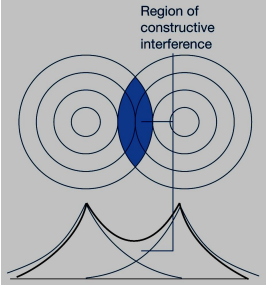
\includegraphics[width=5cm]{fig/lzhx/微信图片_20211102112346.png}
    \caption{$\rho_+$的分布图像}
    \end{minipage}
    \begin{minipage}[t]{0.48\textwidth}
    \centering
    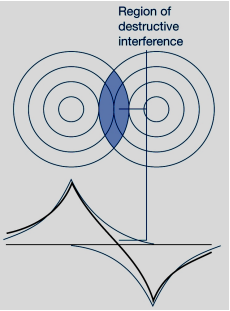
\includegraphics[width=5cm]{fig/lzhx/微信图片_202111021123461.png}
    \caption{$\rho_-$的分布图像}
    \end{minipage}
\end{figure}

有意思的是,如果考虑了重叠积分,组成的分子轨道上升的能量比下降的多:
\[\Delta E=\left(\frac{\alpha-\beta}{1-S}-\alpha\right)-\left(\alpha-\frac{\alpha+\beta}{1+S}\right)=2S \cdot \frac{\alpha S-\beta}{1-S^2}\]

考虑重叠积分$S$一般比较小,做小量分析,原式$\sim 2S \cdot (-\beta)>0$

\section{计算化学入门前的垫脚石上的艹}
\subsection{Hartree-Fock方法}
我们都知道一个孤立微观系统的哈密顿如下:
\[\hat{H}=\hat{T}_N+\hat{T}_e+\hat{V}_{Ne}+\hat{V}_{ee}+\hat{V}_{NN}\]
在BO近似后,$\hat{T}_N$从电子哈密顿中被移除,$\hat{V}_{NN}$给定核位置后是个常数,可以不包含在电子哈密顿中,但一般来说都还是算的。
\[\hat{H}_{el}=\hat{T}_e+\hat{V}_{Ne}+\hat{V}_{ee}+\hat{V}_{NN}=\sum_i\left(-\frac{1}{2}\nabla^2_i+\sum_N\frac{Z}{r_{Ni}}\right)+\sum_{i<j}\frac{1}{r_{ij}}+V_{NN}\]

虽然我们已经把核项给舍去了,但电子部分的哈密顿依然是一个多体哈密顿,还是一个难以求解的问题。
我们一般能处理的都是单体问题,比如氢原子的电子薛定谔、谐振子等等,所以我们希望能将多体问题尽可能精确地转换为单体问题来处理,如我们考虑平均场近似,即将其他电子对该电子的两体作用考虑为一个等效场:
\[\hat{H}_{el} \approx \sum_i\left(-\frac{1}{2}\nabla^2_i+\sum_N\frac{Z}{r_{Ni}}+\hat{v}_i\right)+V_{NN}:=\sum_i\hat{F}_i + V_{NN}\]

如此一来,上述多电子问题就被转换为了单电子问题,多体哈密顿量被转换单体哈密顿量的加和,理所当然,该体系的波函数也变成了几个单体波函数(自旋轨道)的乘积Hartree积:
\[\Psi = \psi_1(1)\psi_2(2)\cdots\psi_n(n)=\prod_i\psi_i(i)\]

由于电子费米子的全同性的要求,上述需要对Hartree基做反对称化得到Slater行列式:
\[\Psi=\frac{1}{\sqrt{n!}}
    \begin{vmatrix}
        u_1(1) & u_2(1) & \ldots & u_n(1)\\
        u_1(2) & u_2(2) & \ldots & u_n(2)\\
        \vdots & \vdots & \ddots & \vdots\\
        u_1(n) & u_2(n) & \ldots & u_n(n)\\
    \end{vmatrix}
\]

可以看到上面我们假定了单体波函数组成的体系波函数是精确的,然后认为哈密顿量是不精确的,由此出发,我们会希望通过不断修正哈密顿量来使得结果更精确,于是就有了MP2、MP4等微扰方法的出现。
另一方面,如果我们认为哈密顿量是精确的,那么就认为波函数是不精确的,从Slater行列式出发我们通过变分方法来求解尽可能精确的波函数,已知能量表达式为:
\[E=\frac{\bra{\Psi}\hat{H}\ket{\Psi}}{\bra{\Psi}\ket{\Psi}}\]

体系波函数满足:
\[\bra{u_i(1)}\ket{u_j(1)}=\delta_{ij}\]

体系哈密顿量为:
\[\hat{H}=\sum_i\left(-\frac{1}{2}\nabla^2_i+\sum_N\frac{Z}{r_{Ni}}\right)+\sum_{i<j}\frac{1}{r_{ij}}+V_{NN}\]

由Condon-Slater规则可知,能量$E$如下所示,其中$\bra{ij}\ket{ij},\bra{ij}\ket{ji}$为库伦积分和交换积分,$\hat{h}_i$包括了动能项和核对电子的势能(单体算符):
\[E=\bra{\varPhi}\hat{H}\ket{\varPhi}=\sum_ih_i+\frac{1}{2}\sum_{i,j}\left(\bra{ij}\ket{ij}-\bra{ij}\ket{ji}\right)\]

得到了能量,我们接下来顺理成章的就该来变分,但这里的变分并不是简单的求极值,而是条件变分,由于波函数的限制我们求变分时需要引入以下条件进行拉格朗日乘数法:
\[\bra{u_i(1)}\ket{u_j(1)}-\delta_{ij}=0\]

定义泛函$\eta(\lambda_{ij})$:
\[\eta(\lambda_{ij})=E+\sum_{i,j}\lambda_{ij}(\bra{u_i(1)}\ket{u_j(1)}-\delta_{ij})\]

由(变分计算量太大而且其他书上有,我就不写了):
\[\frac{\delta\eta(\lambda_{ij})}{\delta u_i}=\frac{\delta}{\delta u_i}\left(E+\sum_{i,j}\lambda_{ij}(\bra{u_i(1)}\ket{u_j(1)}-\delta_{ij})\right)=0\]

得到的变分结果我们记为:
\[\hat{F}\varphi_i=\varepsilon_i\varphi_i \qquad \varepsilon_i=\bra*{u_i}\hat{h} + \hat{J} - \hat{K}\ket*{u_i}\]

其中,$\hat{F}$为Fork算符,$\varepsilon_i$为轨道能量,$\varphi_i$为正则自旋轨道,Fork算符表达式为:
\[\hat{F} = \hat{h} + \hat{J} - \hat{K}\]
\[\hat{J}u_i(1) = \sum_{j \neq i}\left(\int u_j^*(2)\frac{1}{r_{ij}}u_j(2)d\tau_2\right)u_i(1) \qquad \hat{K}u_i(1) = \sum_{j \neq i}\left(\int u_j^*(2)\frac{1}{r_{ij}}u_i(2)d\tau_2\right)u_j(1)\]

Hartree-Fork能量如下给出,可以看到其不等于轨道能量之和,原因是因为考虑了电子之间的相互作用。

\[E_{HF}=\sum_ih_i+\frac{1}{2}\sum_{i,j}\left(\bra{ij}\ket{ij}-\bra{ij}\ket{ji}\right)+V_{NN}\]

当然,单个Slater行列式描述一个多体问题也是有误差的,于是我们希望能进一步地精确波函数,于是就有了CI、CC等方法。

话说回来,由于我们还是给不出每一个自旋轨道的解析式,所以这个方法我们还没办法直接用。

\subsection{Hartree-Fock–Roothaan方法}
如上文所说,我们给不出Hartree-Fock方程所需的体系波函数,所以我们需要用已知的函数去拟合体系波函数,这里给出Roothaan给出的方法,得到的方程称为Hartree-Fock–Roothaan方程:

假定体系波函数可以被已知基组展开,下面的公式中同时会展示矩阵表示,基向量采用行向量表示:
\[\psi_i=\sum_{\nu=1}c_{\nu i}f_{\nu} \qquad (\mathbf{\Psi} = \mathbf{\Phi} \mathbf{C}_{\text{coeff}})\]
将基函数带入Hartree-Fock方程后可以得到如下表达式:
\[\hat{F}\sum_{\nu=1}c_{\nu i}f_{\nu}=\varepsilon_i\sum_{\nu=1}c_{\nu i}f_{\nu}\]
对上述方程等式两边同时左乘一个$f_{\mu}$可以得到
\[\sum_{\nu=1}c_{\nu i}\bra{f_{\mu}}\hat{F}\ket{f_{\nu}}=\varepsilon_i\sum_{\nu=1}c_{\nu i}\bra{f_{\mu}}\ket{f_{\nu}} \quad \text{where} \quad F_{rs}=\bra{f_r}\hat{F}\ket{f_s} \quad \text{and} \quad S_{rs}=\bra{f_r}\ket{f_s}\]

如果把所有波函数都做上述展开,则可写成如下Hartree-Fock–Roothaan方程
\[\mathbf{F}\mathbf{C}=\mathbf{S}\mathbf{C}\varepsilon\]

上述方程组似乎跟我们能解的方程有一点点不一样,我们能处理的是方程组是厄密矩阵(这里是实对称阵)的正交对角化的问题:
\[\mathbf{F}\mathbf{C}'=\mathbf{C}'\varepsilon\]

Fock矩阵也是实对称矩阵,overlap矩阵也是实对称矩阵,我们自然会想到能不能将Hartree-Fock–Roothaan方程转化成上述方程呢?
考虑如下基的酉变换:
\[\phi_i = \sum_{i}U_{ji}f_j \qquad \mathbf{\varPhi}=\mathbf{U}\mathbf{\Psi}\]
其中$\mathbf{U}$为
\[\mathbf{U}=\mathbf{X}\mathbf{s}^{-1/2} \qquad \mathbf{X}^{\dagger}\mathbf{S}\mathbf{X}=\mathbf{s}\]
$\mathbf{X}$,$\mathbf{s}$为$\mathbf{S}$正交对角化的变换矩阵和对角阵,$\mathbf{s}^{-1/2}$为矩阵$\mathbf{s}^{-1}$的开放,其定义为$\mathbf{s}^{-1/2}\mathbf{s}^{-1/2}=\mathbf{s}^{-1}$。

做完如下变换之后,Hartree-Fock–Roothaan方程可以改写成:
\[\mathbf{U}^{\dagger}\mathbf{S}\mathbf{U}\mathbf{C}'=(\mathbf{X}\mathbf{s}^{-1/2})^{\dagger}\mathbf{S}(\mathbf{X}\mathbf{s}^{-1/2})\mathbf{C}'=\mathbf{X}^{\dagger}\mathbf{S}\mathbf{X}\mathbf{s}^{-1}\mathbf{C}'=\mathbf{s}\mathbf{s}^{-1}\mathbf{C}'=\mathbf{C}' \ , \ (\mathbf{C}':=\mathbf{U}^{\dagger}\mathbf{C})\]
\[\mathbf{U}^{\dagger}\mathbf{F}\mathbf{U}\mathbf{C}'=\varepsilon\mathbf{C}' \Rightarrow \mathbf{F}'\mathbf{C}'=\varepsilon\mathbf{C}' \ , \ (\mathbf{F}':=\mathbf{U}^{\dagger}\mathbf{F}\mathbf{U})\]

然后我们就能解这样一个变换后的方程了。
实际上在python中使用scipy.linalg.eigh($\mathbf{F}$,$\mathbf{S}$)就能直接解出$\mathbf{C}$。
但求解Hartree-Fock–Roothaan方程真的只是做一个对角化吗,如果是这样就好了。
我们具体来看每个矩阵的具体形式,系数矩阵和overlap矩阵是简单的,fock矩阵包含了单电子积分和双电子积分:
\[F_{\mu\nu} = \bra*{\phi_{\mu}}\hat{h} + \hat{J} - \hat{K}\ket*{\phi_{\nu}}\]
单电子积分是简单的
\[h_{\mu\nu}=\bra*{\phi_{\mu}}\hat{h}\ket*{\phi_{\nu}}\]
双电子积分我们打包处理
\begin{equation*}
    \begin{aligned}
        \bra*{\phi_{\mu}}\hat{J} - \hat{K}\ket*{\phi_{\nu}} & = \bra*{\phi_{\mu}}\ket{\sum_{j \neq i}\left(\int u_j^*(2)\frac{1}{r_{ij}}u_j(2)\dd{\tau_2}\right)\phi_{\nu}(1)-\sum_{j \neq i}\left(\int u_j^*(2)\frac{1}{r_{ij}}\phi_{\nu}(2)\dd{\tau_2}\right)u_j(1)} \\
         & = \sum_{j}\iint \phi_{\mu}^*(1)u_j^*(2)\left[\frac{1}{r_{ij}}(1-\hat{P}_{12})\right]u_j(2)\phi_{\nu}(1) \dd{\tau_1}\dd{\tau_2} \\
         & = \sum_{\alpha}\sum_{\beta}\sum_{j}c^*_{\alpha j}c_{\beta j}\iint \phi_{\mu}^*(1)\phi_{\alpha}^*(2)\left[\frac{1}{r_{ij}}(1-\hat{P}_{12})\right]\phi_{\beta}(2)\phi_{\nu}(1) \dd{\tau_1}\dd{\tau_2} \\
         & := \sum_{\alpha}\sum_{\beta}D_{\alpha\beta}\iint \phi_{\mu}^*(1)\phi_{\alpha}^*(2)\left[\frac{1}{r_{ij}}(1-\hat{P}_{12})\right]\phi_{\beta}(2)\phi_{\nu}(1) \dd{\tau_1}\dd{\tau_2} \\
         & := \sum_{\alpha}\sum_{\beta}D_{\alpha\beta}\bra{\phi_{\mu}\phi_{\alpha}}\ket{|\phi_{\nu}\phi_{\beta}}
    \end{aligned}
\end{equation*}
其中$D_{\alpha\beta}$是密度矩阵的矩阵元,显然我们知道密度矩阵可以由系数矩阵得到$\mathbf{D}=\mathbf{C}\mathbf{C}^{\dagger}$,所以事实上,我们得到的类似矩阵对角化的一个方程实际上也不像是看起来的那么简单,对这样的方程我们没办法直接求解,于是我们选择万能的迭代。
迭代需要一个初猜,在这里也就是初始的密度矩阵(给初猜也是技术活),然后通过对角化更新密度矩阵,反复迭代直到密度矩阵不再变化,这也就是SCF过程。
\[\mathbf{F}(\mathbf{C}')\mathbf{C}'=\mathbf{C}'\varepsilon\]

关于Hartree-Fock方法更多的内容推荐大家阅读\textbf{Szabo前三章},也希望各位能够自己写一个程序来实现(doge),这里提供两个实例:
\href{https://github.com/yangdatou/hf-tutorial}{大头版HF (积分算好了) }和
\href{https://github.com/Walter-Feng/Hartree-Fock-in-CPP}{叔叔版HF (从基组开始嗯造)}。

Hartree-Fock–Roothaan方程还有另外一个形式,以密度矩阵形式体现
\[\mathbf{F}\mathbf{P}\mathbf{S}=\mathbf{S}\mathbf{P}\mathbf{F}\]

证明上述方程与Hartree-Fock–Roothaan方程等价之前先介绍密度矩阵的几个性质
\[1. \ \mathbf{P}=\mathbf{P}^{\dagger} \qquad 2. \ \mathbf{P}\mathbf{S}\mathbf{P}=\mathbf{P} \qquad 3.\ \text{Tr}(\mathbf{P}\mathbf{S})=N\]

开始证明
\[\mathbf{F}\mathbf{C}=\varepsilon\mathbf{S}\mathbf{C} \quad \Rightarrow \quad \mathbf{F}\mathbf{C}(\mathbf{S}\mathbf{C})^{\dagger}=\varepsilon\mathbf{S}\mathbf{C}(\mathbf{S}\mathbf{C})^{\dagger} \quad \Rightarrow \quad \mathbf{F}\mathbf{P}\mathbf{S}=\varepsilon\]
\[\mathbf{F}\mathbf{C}=\varepsilon\mathbf{S}\mathbf{C} \quad \Rightarrow \quad \mathbf{F}\mathbf{C}(\mathbf{F}\mathbf{C})^{\dagger}=\varepsilon\mathbf{S}\mathbf{C}(\mathbf{F}\mathbf{C})^{\dagger} \quad \Rightarrow \quad \mathbf{I}=\varepsilon\mathbf{S}\mathbf{P}\mathbf{F} \quad \Rightarrow \quad \mathbf{I}=(\varepsilon\mathbf{S}\mathbf{P}\mathbf{F})^{\dagger} \quad \Rightarrow \quad \mathbf{S}\mathbf{P}\mathbf{F}=\varepsilon^{\dagger}=\varepsilon\]

基于上述形式的自洽场方程可以介绍DIIS辣!


\subsection{部分基组}
\paragraph*{Slater-type orbitals (STO's)}
\[\phi_{abc}^{STO}(x,y,z)=Nx^ay^bz^ce^{-\zeta r}\]
其中,$N$为归一化系数,且a,b,c被角动量控制:$a+b+c=L$,在远距离与近距离行为拟合实际波函数较好。长得跟氢原子波函数形式相近但是缺乏节点且不完全球谐,且收敛慢。

\paragraph*{Gaussian-type orbitals (GTO's)}
\[\phi_{abc}^{GTO}(x,y,z)=Nx^ay^bz^ce^{-\zeta r^2}\]
其中,$N$为归一化系数,且a,b,c被角动量控制:$a+b+c=L$。收敛快且有多种方法处理,长得跟氢原子波函数完全不一样。单个函数在近距离行为相较于Slater函数拟合实际波函数较差,解决办法是用多个函数来逼近Slater函数。

\begin{center}
    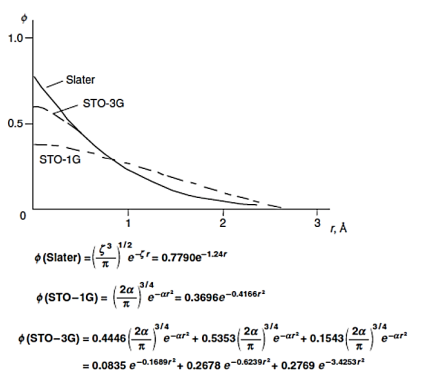
\includegraphics{fig/lzhx/微信图片_20211102165150}
\end{center}

\paragraph*{Contracted Gaussian type orbitals (CGTO's)}
\[\phi_{abc}^{CGTO}(x,y,z)=N\sum_{i=1}^n x^ay^bz^ce^{-\zeta r^2}\]
比较神奇的是,一般我们不叫这个基组CGTO,而是STO-nG。

下面给出的是STO-3G描述不同原子需要的函数个数,一般而言STO-3G都是作为计算体系的极小基:
\begin{center}
    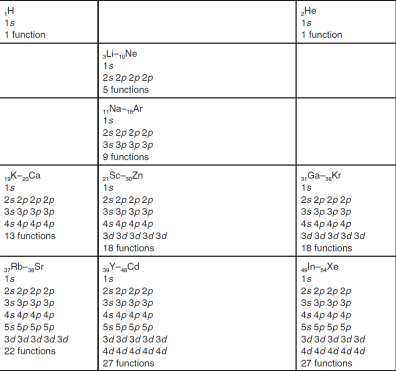
\includegraphics[scale=0.7]{fig/lzhx/微信图片_20211102171332.png}
\end{center}

\paragraph*{3–21G Split Valence and Double-Zeta Basis Set}
在这种基组下,我们把电子分为两种,核层(core orbitals)与价层(valence orbital),内层的轨道每一个轨道用一个包含三个Gaussian函数的基函数描述,价层每个轨道分为内层与外层,内层(inner shell)用两个Gaussian函数描述,外层(outer shell)用一个Gaussian函数描述,6-31G等同理:
\begin{center}
    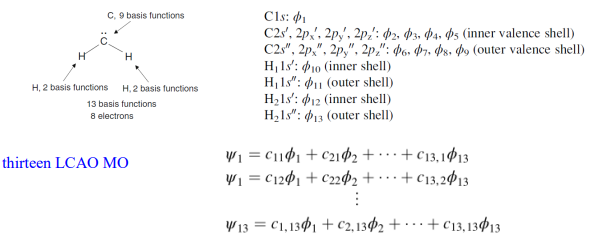
\includegraphics[scale=0.9]{fig/lzhx/微信图片_20211102172815}
\end{center}
\begin{center}
    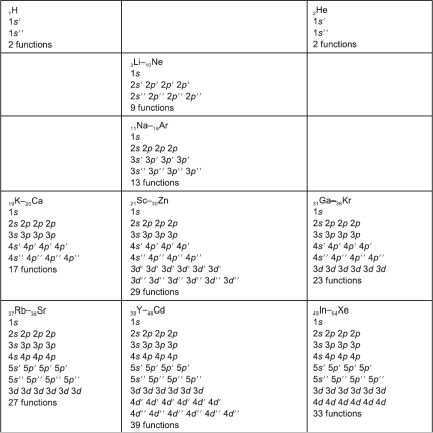
\includegraphics[scale=0.7]{fig/lzhx/微信图片_202111021728151}
\end{center}

\section{分子光谱}
在化学范围内,我们考虑一个分子的能量由平动、转动、振动、电子能量组成:
\[E=E_{tr}+E_{rot}+E_{vib}+E_{ele}\]
\begin{center}
    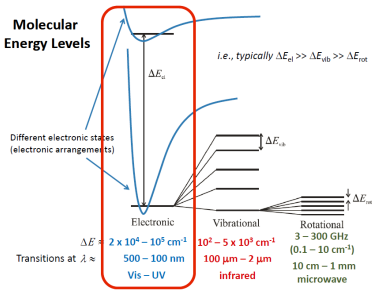
\includegraphics{fig/lzhx/微信图片_20211102175446.png}
\end{center}

与原子光谱类似,分子光谱也有类似的表达方式:
\[M^S\Lambda^{(+/-)}_\Omega\]

其中,$s$、$\Lambda$、$\Omega$由下式给出:
\[S=2s+1 \qquad \hat{J}_z\varPsi=\Lambda\varPsi \qquad \Omega=|\Lambda+S| \qquad \Lambda=\sum_ij_i \qquad S=\sum_iS_i\]

$\Lambda$的取值如下,判断的方法是看开壳层电子所在轨道的$j$值的矢量叠加:
\[\begin{array}{ll}
    \Lambda=0 & \Sigma \\
    \Lambda=\pm 1 & \Pi \\
    \Lambda=\pm 2 & \Delta \\
    \cdots
\end{array}\]

$\Omega$的结果通常用$g$或者$u$来表示,其取值可以通过判断$u$轨道上的单电子个数来判断——每一个在$u$上的电子其对称性都记为$u$,总的$\Omega$取值通过以下方式将各个$u$通过结合运算合成:
\begin{center}
    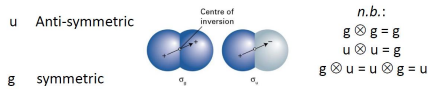
\includegraphics{fig/lzhx/微信图片_20211106011930.png}
\end{center}

分子谱相中右上角的角标$+/-$仅在$\Lambda$取值为$\Sigma$时显现,其取值由波函数轨道部分对称或反对称决定:对称时为+,反之为-。

$M$为按能量从低到高用符号$X$、$A$、$B$$\cdots$来表示,如:$X^3\Sigma^-_g$、$A^1\nabla^2_g$、$B^1\Sigma^+_g$。

谱相的多重度为:
\[
    \begin{array}{ll}
        2(2s+1) & if \quad \Lambda \neq 0 \\
        2s+1 & if \quad \Lambda = 0
    \end{array}
\]

\subsection{双原子分子光谱实例}
如果不考虑将电子激发到其他能级上,$O_2$分子可能的开壳层排布为:
\[
    \begin{array}{lcccccc}
        state & \pi_+(\alpha\beta)\pi_- & \pi_+(\alpha)\pi_-(\alpha) & \pi_+(\alpha)\pi_-(\beta) & \pi_+(\beta)\pi_-(\alpha) & \pi_+(\beta)\pi_-(\beta) & \pi_+\pi_-(\alpha\beta) \\
        M_L=  & 2 & 0 & 0 & 0 & 0 & -2 \\
        M_S=  & 0 & 1 & 0 & 0 & -1 & 0
    \end{array}
\]

当然,这么写是并不完全合理,由于全同性,对于对应相同谱相的电子组态我们无法区分,如1、6,3、4三对电子组态,因此,在正式确定对应于同一个谱相的电子组态时,我们需要按照波函数反对称化以及粒子全同性的要求将其两两线性组合。

如对1、6这组,首先写出其价层的$Slater$行列式,并定义简写:
\[
\varphi_1=\frac{1}{\sqrt{2}}
\begin{vmatrix}
    \pi_{g+}(1)\alpha(1) & \pi_{g+}(1)\beta(1) \\
    \pi_{g+}(2)\alpha(2) & \pi_{g+}(2)\beta(2)
\end{vmatrix}
:=
\begin{vmatrix}
    \pi_{g+}(1)\alpha(1) & \pi_{g+}(2)\beta(2)
\end{vmatrix}
\]
\[
\varphi_6=\frac{1}{\sqrt{2}}
\begin{vmatrix}
    \pi_{g-}(1)\alpha(1) & \pi_{g-}(1)\beta(1) \\
    \pi_{g-}(2)\alpha(2) & \pi_{g-}(2)\beta(2)
\end{vmatrix}
:=
\begin{vmatrix}
    \pi_{g-}(1)\alpha(1) & \pi_{g-}(2)\beta(2)
\end{vmatrix}
\]

由于我们指定了这两个电子排布在某个确定角动量的轨道上,这不符合粒子全同性的要求,当然更本质的原因是这两个波函数不是$\hat{S}^2$的本征函数,其自旋无意义,这里需要对两个态进行正交线性组合:
\[\Psi=\frac{1}{\sqrt{2}}(\varphi_1+\varphi_6) \qquad \Psi'=\frac{1}{\sqrt{2}}(\varphi_1-\varphi_6)\]

\[|M_L|=2 \qquad |M_S|=0 \qquad g \times g=g\]

故,这两组电子组态对应的分子谱项为:$^1\nabla^2_g$

同理,对2、5组:
\[
\varphi_2=\frac{1}{\sqrt{2}}
\begin{vmatrix}
    \pi_{g+}(1)\alpha(1) & \pi_{g-}(1)\alpha(1) \\
    \pi_{g+}(2)\alpha(2) & \pi_{g-}(2)\alpha(2)
\end{vmatrix}
=\frac{1}{\sqrt{2}}
\begin{vmatrix}
    \pi_{g+}(1) & \pi_{g-}(1) \\
    \pi_{g+}(2) & \pi_{g-}(2)
\end{vmatrix}
\alpha(1)\alpha(2)
\]
\[
\varphi_5=\frac{1}{\sqrt{2}}
\begin{vmatrix}
    \pi_{g+}(1)\beta(1) & \pi_{g-}(1)\beta(1) \\
    \pi_{g+}(2)\beta(2) & \pi_{g-}(2)\beta(2)
\end{vmatrix}
=\frac{1}{\sqrt{2}}
\begin{vmatrix}
    \pi_{g+}(1) & \pi_{g-}(1) \\
    \pi_{g+}(2) & \pi_{g-}(2)
\end{vmatrix}
\beta(1)\beta(2)
\]

这两种状态并不违反粒子全同性,故无需重新线性组合,他们对应相同的光谱项。
\[|M_L|=0 \qquad |M_S|=2 \qquad g \times g=g\]

由于轨道波函数部分反对称,故,这两组电子组态对应的分子谱项为:$^3\Sigma_g^-$

对3、4组:
\[
\varphi_3=\frac{1}{\sqrt{2}}
\begin{vmatrix}
    \pi_{g+}(1)\alpha(1) & \pi_{g-}(1)\alpha(1) \\
    \pi_{g+}(2)\beta(2) & \pi_{g-}(2)\beta(2)
\end{vmatrix}
=\frac{1}{\sqrt{2}}
\begin{vmatrix}
    \pi_{g+}(1) & \pi_{g-}(1) \\
    \pi_{g+}(2) & \pi_{g-}(2)
\end{vmatrix}
\alpha(1)\beta(2)
\]
\[
\varphi_4=\frac{1}{\sqrt{2}}
\begin{vmatrix}
    \pi_{g+}(1)\beta(1) & \pi_{g-}(1)\beta(1) \\
    \pi_{g+}(2)\alpha(2) & \pi_{g-}(2)\alpha(2)
\end{vmatrix}
=\frac{1}{\sqrt{2}}
\begin{vmatrix}
    \pi_{g+}(1) & \pi_{g-}(1) \\
    \pi_{g+}(2) & \pi_{g-}(2)
\end{vmatrix}
\beta(1)\alpha(2)
\]

显然,这样的排布不满足全同性的要求,重新线性组合得到:
\[\Psi=\frac{1}{2}(\pi_{g+}(1)\pi_{g-}(2)-\pi_{g-}(1)\pi_{g+}(2))(\alpha(1)\beta(2)+\beta(1)\alpha(2))\]
\[\Psi'=\frac{1}{2}(\pi_{g+}(1)\pi_{g-}(2)+\pi_{g-}(1)\pi_{g+}(2))(\alpha(1)\beta(2)-\beta(1)\alpha(2))\]
\[|M_L|=0 \qquad |M_S|=2 \qquad g \times g=g\]

考虑轨道部分,对$\Psi$,其最外层轨道部分反对称,故右上角表为-,同理$\Psi$右上角表为+,注意到$\Psi$的自选部分为三重态,故其左上角标为3而非单重态的1:
\[
    \begin{array}{ll}
        \Psi & ^3\Sigma_g^- \\
        \Psi' & ^1\Sigma_g^+ 
    \end{array}
\]

最后,按能量高低给氧分子的三个谱相表上相应符号:
\begin{center}
    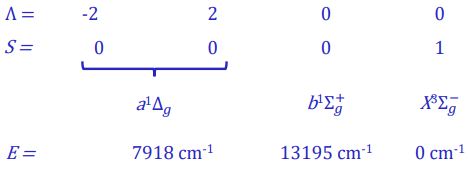
\includegraphics{fig/lzhx/微信图片_20211106140136.png}
\end{center}

\section{附录I:氢原子薛定谔方程求解(级数解法)}
利用分离变量法,我们假定定态波函数$\varPsi(r,\theta,\varphi)$可以表示成如下形式:
\[\varPsi(r,\theta,\varphi)=R(r)\Theta(\theta)\varPhi(\varphi)\]

带入定态薛定谔方程:
\[\hat{H}R(r)\Theta(\theta)\varPhi(\varphi)=ER(r)\Theta(\theta)\varPhi(\varphi)\]

将哈密顿算符展开,将拉普拉斯算符在极坐标系下展开,并整理方程,我们可以得到:
\[\frac{\Theta\varPhi}{r^2}\frac{\partial}{\partial{r}}(r^2\frac{\partial R}{\partial{r}})+\frac{R\varPhi}{r^2sin\theta}\frac{\partial}{\partial{\theta}}(sin\theta\frac{\partial \Theta}{\partial{\theta}})+\frac{R\Theta}{r^2sin^2 \theta }\frac{\partial^2 \varPhi}{\partial{\phi^2}}=-\frac{2m(E-V)}{\hbar^2}R\Theta\varPhi\]

在方程两边同时乘上因子$\frac{r^2sin^2 \theta}{R\Theta\varPhi}$,我们可以得到:
\[\frac{sin^2 \theta}{R}\frac{\partial}{\partial{r}}(r^2\frac{\partial R}{\partial{r}})+\frac{sin\theta}{\Theta}\frac{\partial}{\partial{\theta}}(sin\theta\frac{\partial \Theta}{\partial{\theta}})+\frac{1}{\varPhi}\frac{\partial^2 \varPhi}{\partial{\phi^2}}=-\frac{2m(E-V)}{\hbar^2}r^2sin^2 \theta\]

再通过移向,我们得到:
\[\frac{sin^2 \theta}{R}\frac{\partial}{\partial{r}}(r^2\frac{\partial R}{\partial{r}})+\frac{sin\theta}{\Theta}\frac{\partial}{\partial{\theta}}(sin\theta\frac{\partial \Theta}{\partial{\theta}})+\frac{2m(E-V)}{\hbar^2}r^2sin^2 \theta=-\frac{1}{\varPhi}\frac{\partial^2 \varPhi}{\partial{\phi^2}}\]

由于方程两边变量不同,若满足上述等式,方程左右两边都应等于同一个常数,不妨假设该常数为$m^2$,则我们可以得到两个方程:
\[\frac{\partial^2 \varPhi}{\partial{\phi^2}}+m^2\varPhi=0 \tag{a}\]
\[\frac{sin^2 \theta}{R}\frac{\partial}{\partial{r}}(r^2\frac{\partial R}{\partial{r}})+\frac{sin\theta}{\Theta}\frac{\partial}{\partial{\theta}}(sin\theta\frac{\partial \Theta}{\partial{\theta}})+\frac{2m(E-V)}{\hbar^2}r^2sin^2 \theta=m^2 \tag{4}\]

将方程$4$两边同时除以$sin^2 \theta$并整理,我们得到:
\[\frac{1}{R}\frac{\partial}{\partial{r}}(r^2\frac{\partial R}{\partial{r}})+\frac{2m(E-V)}{\hbar^2}r^2=\frac{m^2}{sin^2 \theta}-\frac{1}{\Theta sin\theta}\frac{\partial}{\partial{\theta}}(sin\theta\frac{\partial \Theta}{\partial{\theta}})\]

同样的,我们假定上述方程左右两边均等于参数$\beta$,于是我们又得到两个方程:
\[\frac{1}{R}\frac{\partial}{\partial{r}}(r^2\frac{\partial R}{\partial{r}})+\frac{2m(E-V)}{\hbar^2}r^2=\beta \tag{b}\]
\[\frac{m^2}{sin^2 \theta}-\frac{1}{\Theta sin\theta}\frac{\partial}{\partial{\theta}}(sin\theta\frac{\partial \Theta}{\partial{\theta}})=\beta \tag{c}\]

至此,我们将定态薛定谔方程拆分成三个含不同变量的常微分方程$a,b,c$。
\subsection{Φ方程的求解}
由球坐标中$\varphi$的范围及其边界条件$\varPhi(x)=\varPhi(x+2\pi)$、归一化条件以及方程$a$,我们在这一小节将要处理的对象是柯西问题:
\[\frac{\mathrm{d}^2 \varPhi}{\mathrm{d}{\phi^2}}+ m^2 \varPhi=0 \qquad \varPhi(x)=\varPhi(x+2\pi) ,\int_{0}^{2\pi}\varPhi^{*}\varPhi d\phi=1\]

方程$a$的通解形式为:
\[\varPhi(\phi)=C_1 e^{im\phi}+C_2 e^{-im\phi}\]

带入上述边界条件,我们得到上述柯西问题的解:
\[\varPhi(\phi)=\frac{1}{\sqrt{2\pi}}e^{im\phi} \qquad (m=0,\pm 1,\pm 2\cdot\cdot\cdot)\]

但显然,上述解与方程$a$的通解并不相同。但问题不大,由于微分方程特解的线性叠加性,我们可以选取一对绝对值为$|m|$的解线性叠加成我们认知中的方程$a$的通解。

\subsection{Θ方程的求解}
对方程$c$,我们做以下代换:
\[x=cos\theta \qquad \frac{\mathrm{d} \Theta}{\mathrm{d} x}=\frac{\mathrm{d} \Theta}{\mathrm{d} \theta}\left ( \frac{\mathrm{d} x}{\mathrm{d} \theta} \right )^{-1}=-\frac{1}{sin\theta} \frac{\mathrm{d} \Theta}{\mathrm{d} \theta} \qquad y(x)=\Theta(\theta)\]

则方程$c$可以改写成以下形式:
\[\frac{m^2}{1-x^2}-\frac{1}{y}\frac{\mathrm{d}}{\mathrm{d}{x}} \left [(1-x^2) \frac{\mathrm{d} y}{\mathrm{d}{x}} \right ]=\beta\]

经整理,我们可以将上述方程改写成:
\[\frac{\mathrm{d}}{\mathrm{d}{x}} \left [(1-x^2) \frac{\mathrm{d} y}{\mathrm{d}{x}} \right ]+\left (\beta- \frac{m^2}{1-x^2} \right )y=0\]

上述方程即为连带$Legendre$方程。

为了求解上述方程,我们需要从其简化入手,下面我们将给出连带$Legendre$方程的简化,$Legendre$方程:
\[\frac{\mathrm{d}}{\mathrm{d}{x}} \left [(1-x^2) \frac{\mathrm{d} y}{\mathrm{d}{x}} \right ]+\beta y=0\]

我们将用级数解法求解该方程,为了保证级数解法的正确性,我们引用一下定理保证在我们给定条件下的$Legendre$方程的解存在且唯一:

\textbf{定理} \qquad 如果$p(z)$和$q(z)$在圆$|z-z_0|<R$内单值解析,则在此圆内二阶线性微分方程的初值问题:
\[\frac{\mathrm{d}^2w}{\mathrm{d}x^2}+p(z)\frac{\mathrm{d}w}{\mathrm{d}x}+q(z)w=0\]
\[w(z_0)=a \qquad w^{'}(z_0)=b \qquad (\forall a,b \in \mathbb{C})\]
的解存在且唯一,并且解$w(z)$在这个圆内单值解析。

下面我们将开始求解$Legendre$方程,其中自变量$x$定义在$[-1,1] \subset \mathbb{R}$,我们首先取$x_0=0$,显然0是$Legendre$方程的常点,因此,我们假设方程的解在$x_0=0$的邻域内可以展开成一下形式:
\[y=\sum_{k=0}^{+\infty}c_kx^k\]

将展开式带入$Legendre$方程,并整理,我们得到:
\[\sum_{k=0}^{+\infty} \left \{ (k+2)(k+1)c_{k+2}-[k(k+1)-\beta]c_k \right \}x^k=0\]

然后我们得到了递推关系:
\[c_{k+2}=\frac{k(k+1)-\beta}{(k+2)(k+1)}c_k\]

进而:
\[c_{2k}=\prod_{n=1}^{k}\frac{(2k-1)(2k-2)-\beta}{(2k)(2k-1)}c_0\]
\[c_{2k+1}=\prod_{n=1}^{k}\frac{(2k)(2k-1)-\beta}{(2k)(2k+1)}c_1\]

因此,我们可以将方程的解按奇偶项拆开:
\[y(x)=c_1y_0(x)+c_2y_1(x)\]
\[y_0(x)=1+\sum_{k=1}^{+\infty}\frac{c_{2k}}{c_0}x^{2k}\]
\[y_1(x)=x+\sum_{k=1}^{+\infty}\frac{c_{2k+1}}{c_1}x^{2k+1}\]

容易看出当x取值$x= \pm 1$时,无穷级数$y_0(x)$、$y_1(x)$发散,与边界条件$|y(\pm 1)|< +\infty$矛盾,为了解决这个问题,我们将要使得无穷级数$y_0(x)$、$y_1(x)$退化为有限项,为此,我们将对特征值$\lambda$赋值:
\[\beta=l(l+1) \qquad l \in \mathbb{N}_{+}\]
\[y_0(x)=\sum_{k=0}^{+\infty}\frac{2^{2k}}{(2k)!}\frac{\Gamma(k-\frac{l}{2})\Gamma(\frac{l+1}{2}+k)}{\Gamma(-\frac{l}{2})\Gamma(\frac{l+1}{2})}x^{2k}\]
\[y_0(x)=\sum_{k=0}^{+\infty}\frac{2^{2k}}{(2k+1)!}\frac{\Gamma(k-\frac{l-1}{2})\Gamma(\frac{l}{2}+1+k)}{\Gamma(-\frac{l-1}{2})\Gamma(\frac{l}{2}+1)}x^{2k+1}\]

此时,无穷级数$y(x)$退化成2l项的有限级数$P_l(x)$,我们得到了该方程的本征函数解,也即$Legendre$多项式,在定义域内收敛:
\[P_l(x)=\sum_{k=0}^{[l/2]}(-1)^k \frac{(2l-2k)!}{2^l k! (l-k)!(l-2k)!}x^{l-2k}\]

回到连带$Legendre$方程,我们容易求出方程在$x= \pm 1$与$x=\infty$的指标为$\rho= \pm \frac{m}{2}$,于是我们做以下代换:
\[y=(x^2-1)^{\frac{m}{2}}v(x)\]

带入连带$Legendre$方程展开整理得:
\[(1-x^2)v^{''}-2(m+1)xv^{'}+[\beta-m(m+1)]v=0 \tag{d}\]

如果我们对$Legendre$方程求m次导:
\[\frac{\mathrm{d^{m+1}}}{\mathrm{d}{x^{m+1}}} \left [(1-x^2) \frac{\mathrm{d} y}{\mathrm{d}{x}} \right ]+\beta y^{(m)}=0\]
\[(1-x^2)\frac{\mathrm{d^{m+2}}y}{\mathrm{d}{x^{m+2}}}-2(m+1)x\frac{\mathrm{d^{m+1}}y}{\mathrm{d}{x^{m+1}}}+[\beta-m(m+1)]\frac{\mathrm{d^{m}}y}{\mathrm{d}{x^{m}}}=0\]

发现其与方程d形式相同。

于是,我们能直接写出连带$Legendre$方程的解:
\[y=(x^2-1)^{\frac{m}{2}}\frac{\mathrm{d^{m}}P_l(x)}{\mathrm{d}{x^{m}}}=(x^2-1)^{\frac{m}{2}}\frac{\mathrm{d^{m}}}{\mathrm{d}{x^{m}}}\sum_{k=0}^{[l/2]}(-1)^k \frac{(2l-2k)!}{2^l k! (l-k)!(l-2k)!}x^{l-2k}:=(x^2-1)^{\frac{m}{2}}P^m_l(x)\]

至此,方程b的解可以写成:
\[\Theta(\theta)=(-1)^msin^m(\theta)P^m_l(cos\theta)\]

同时为了满足归一化条件e,$\Theta(\theta)$最终可以表示成:
\[\int_0^{\pi}\Theta_{l,m}^{*}(\theta)\Theta_{l^{'},m^{'}}(\theta)sin\theta d\theta=\nabla^2_{l,l^{'}} \cdot \nabla^2_{m,m^{'}} \tag{e}\]
\[\Theta_{l,m}(\theta)=\sqrt{\frac{(2l-1)(l-|m|)!}{2(l+|m|)!}}P^{m}_l(cos\theta) \qquad |m| \leqslant l\]

此外,$Legendre$多项式也可以通过$Rodrigue$公式定义:
\[P_l(x) \equiv \frac{1}{2^ll!} \left ( \frac{\mathrm{d}}{\mathrm{d}x} \right )^l(x^2-1)^l\]

\textbf{补充说明:本小节涉及到的$m$为加说明均取绝对值。}

\subsection{R方程的求解}

对方程b,我们要处理的是以下柯西问题:
\[\frac{1}{R}\frac{\partial}{\partial{r}}(r^2\frac{\partial R}{\partial{r}})+\frac{2m(E-V)}{\hbar^2}r^2=\beta \qquad r>0 \qquad V=-\frac{e}{4 \pi \varepsilon_0 r}\]

对上述柯西问题,我们做以下代换并整理可以得到方程:
\[u \equiv rR\]
\[-\frac{\hbar^2}{2m}\frac{\mathrm{d^2}u}{\mathrm{d}r^2}+ \left (\frac{\hbar^2}{2m}\frac{l(l+1)}{r^2}-\frac{e}{4 \pi \varepsilon_0r} \right )u=Eu\]

容易看出,当$r \rightarrow +\infty$时,
\[u=Ae^{-\frac{\sqrt{-2mE}}{\hbar}r}+Be^{\frac{\sqrt{-2mE}}{\hbar}r}\]

当$E>0$时,容易看出u不收敛于0,为非束缚态;当$E<0$时,我们可以取$B=0$使得当$r \rightarrow +\infty$时$u \rightarrow 0$,因此,我们取$E<0$。

继续通过代换简化方程形式:
\[\kappa \equiv \frac{\sqrt{-2mE}}{\hbar} \qquad \rho \equiv \kappa r \qquad \rho_o \equiv \frac{me^2}{2 \pi \varepsilon_0 \hbar^2 \kappa}\]
\[\frac{\mathrm{d^2}u}{\mathrm{d}\rho^2}=\left [ 1-\frac{\rho_0}{\rho}+\frac{l(l+1)}{\rho^2} \right ]u\]

当$\rho \rightarrow +\infty$,原方程近似为:
\[\frac{\mathrm{d^2}u}{\mathrm{d}\rho^2}=u\]

其解为:
\[u(\rho)=Ae^{-\rho}+Be^{\rho}\]

由$\lim_{\rho \rightarrow +\infty}u(\rho)=0$,得到$B=0$,最终解应近似为:
\[u(\rho) \sim Ae^{-\rho}\]

当$\rho \rightarrow 0$,原方程近似为:
\[\frac{\mathrm{d^2}u}{\mathrm{d}\rho^2}=\frac{l(l+1)}{\rho^2}u\]

可以验证其解为:
\[u(\rho)=C\rho^{l+1}+D\rho^{-l}\]

由$\lim_{\rho \rightarrow 0}u(\rho)=0$,得到$D=0$,最终解应近似为:
\[u(\rho) \sim C\rho^{l+1}\]

由于$\rho \rightarrow +\infty$与$\rho \rightarrow 0$均在定义域范围内。所以最终$u(\rho)$的解应包含上述的两个部分,不妨假设$u(\rho)$为以下形式:
\[u(\rho)=\rho^{l+1}e^{-\rho}v(\rho)\]

于是,原方程可以展开为:
\[\rho\frac{\mathrm{d^2}v}{\mathrm{d}\rho^2} +2(l+1-\rho)\frac{\mathrm{d}v}{\mathrm{d}\rho}+[\rho_0-2(l+1)]v=0 \]

假定$v(\rho)$可以展开成如下泰勒级数:
\[v(\rho)=\sum_{j=0}^{+\infty}c_j\rho^j\]

则原方程可以展开成:
\[\sum_{j=0}^{+\infty}j(j+1)c_{j+1}\rho^j+2(l+1)\sum_{j=0}^{+\infty}(j+1)c_{j+1}\rho^j-2\sum_{j=0}^{+\infty}jc_j\rho^j+[\rho_0-2(l+1)]\sum_{j=0}^{+\infty}c_j\rho^j=0\]

由于$\rho$取值的任意性,上述方程同阶项系数和应为0,即:
\[j(j+1)c_{j+1}+2(l+1)(j+1)c_{j+1}-2jc_j+[\rho_0-2(l+1)]c_j=0\]

整理得到:
\[c_{j+1}=\frac{2(l+1+j)-\rho_0}{(j+1)(j+2l+2)}c_j\]

对上述递推关系做估计,当$j \rightarrow +\infty$,有:
\[c_{j+1}=\frac{2(l+1+j)-\rho_0}{(j+1)(j+2l+2)}c_j \sim \frac{2j}{(j+1)j}c_j=\frac{2}{(j+1)}c_j\]

那么我们将可以得到:
\[c_j \sim \frac{2^j}{j!}c_0\]
\[v(\rho) \sim c_0\sum_{j=0}^{+\infty}\frac{2^j}{j!}\rho^j=c_0e^{2\rho}\]
\[u(\rho) \sim c_0\rho^{l+1}e^{\rho}\]

可以看出,当$v(\rho)$3为无穷级数时,$u(\rho)$发散,为了解决这个问题,我们可以同样利用上一小节的思路,将无穷级数截断使之退化成有限项级数,保证其收敛性,因此必然存在一个$j_{max}$使得:
\[c_{j_{max}+1}=\frac{2(l+1+j_{max})-\rho_0}{(j_{max}+1)(j_{max}+2l+2)}c_{j_{max}}=0\]

即:
\[2(l+1+j_{max})-\rho_0=0\]

这时,我们定义:
\[n \equiv l+1+j_{max}\]

此时,无穷级数$v(\rho)$退化成了$n-l$项的有限项级数:
\[v(\rho)=L_{n-l-1}^{2l+1}(2\rho)\]

其中$L_q(x)$为$Laguerre$多项式,$L_{q-p}^{p}(x)$为连带$Laguerre$多项式:
\[L_{q-p}^{p}(x)=(-1)^p \left ( \frac{\mathrm{d}}{\mathrm{d}x} \right )^qL_q(x)\]\
\[L_q(x)=e^x\left ( \frac{\mathrm{d}}{\mathrm{d}x} \right )^q(e^{-x}x^q)\]

这里的n也就是主量子数,从其定义式上我们可以很明显得看出角量子数的取值应为:
\[l=0,1,2, \cdot\cdot\cdot ,n-1\]

我们也能看出:
\[\rho_0=2n\]

再结合$\rho_0$与$\kappa$的定义式,我们可以得到:
\[E_n=- \left [\frac{m}{2\hbar^2} \left ( \frac{e^2}{4 \pi \varepsilon_0} \right )^2 \right ] \frac{1}{n^2}\]

以及玻尔半径$a$:
\[\frac{4 \pi \varepsilon_0 \hbar^2}{me^2}=0.529 \times 10^{-10}m\]

最终,再根据归一化条件,我们可以写出方程b的解$R(r)$:
\[R(r)=\sqrt{ \left (\frac{2}{na} \right )^3 \frac{(n-l-1)!}{2n[(n+l)!]^3}}e^{-\frac{r}{na}}\left (\frac{2r}{na} \right )^l \left [L_{n-l-1}^{2l+1} \left ( \frac{2r}{na} \right ) \right ]\]

至此,上述通过分离变量得到的三个方程全部解出。

\subsection{小结}
汇总一下上述三个方程的解:
\[R_{n,l}(r)=\sqrt{ \left (\frac{2}{na} \right )^3 \frac{(n-l-1)!}{2n[(n+l)!]^3}}e^{-\frac{r}{na}}\left (\frac{2r}{na} \right )^l \left [L_{n-l-1}^{2l+1} \left ( \frac{2r}{na} \right ) \right ]\]
\[\Theta_{l,m}(\theta)=\sqrt{\frac{(2l-1)(l-|m|)!}{2(l+|m|)!}}P^{m}_l(cos\theta)\]
\[\varPhi_{m}(\phi)=\frac{1}{\sqrt{2\pi}}e^{im\phi}\]

两个角度变量函数还能合并为$Y_l^m(\theta,\phi)$:
\[Y_l^m(\theta,\phi)=\varepsilon \sqrt{\frac{(2l-1)(l-|m|)!}{4 \pi (l+|m|)!}}e^{im\phi}P^{m}_l(cos\theta)\]

其中,当$m \geq 0$时$\varepsilon=(-1)^m$,当$m \leq 0$时$\varepsilon=1$,以满足其自动正交性。

因此,氢原子定态波函数的解$\varPsi_{n,l,m}$为:
\[\varPsi_{n,l,m}=\sqrt{ \left (\frac{2}{na} \right )^3 \frac{(n-l-1)!}{2n[(n+l)!]^3}}e^{-\frac{r}{na}}\left (\frac{2r}{na} \right )^l \left [L_{n-l-1}^{2l+1} \left ( \frac{2r}{na} \right ) \right ]Y_l^m(\theta,\phi)\]